\chapter{MATERIALS AND METHODS (Yeast8)}

\section{Consensus \emph{S. cerevisiae} Metabolic Model}
Variety of \emph{S. cerevisiae} genome-scale metabolic models have been used since 2003, and each reconstructed model introduced more manual curations, increasing gene numbers from annotations and better predictions regarding the previous ones \cite{lopes2017genome}. A consensus genome-scale metabolic model of \emph{S. cerevisiae}, Yeast8, is presented in an open-source, version-controlled maintainable way in 2019, claiming that the model can be represented and investigated in a systematic way using Git (https://git-scm.com/) and GitHub (https://github.com/) as a hosting service for the model repository \cite{lu2019consensus}. Systematic way of Yeast8 enables to study simultaneously in collaborative studies, provides record keeping of model changes, version updates, where each version of can be released periodically and accessible all the time (Figure \ref{fig:yeast8_github}).

Yeast8 model can be considered as an updated version of Yeast7 \cite{aung2013revising} with additional corrections based on the annotations available in KEGG and ChEBI, and several gene inclusions from the model iSce926 \cite{chowdhury2015using}. Final version of Yeast8, version 8.3.4 released on July 28, has 3991 reactions, 2691 metabolites, 1149 genes, 14 intracellular compartments. Additional statistical analysis results can be seen in Figure \ref{fig:modelstats}.

\begin{figure}[H]
\begin{center}
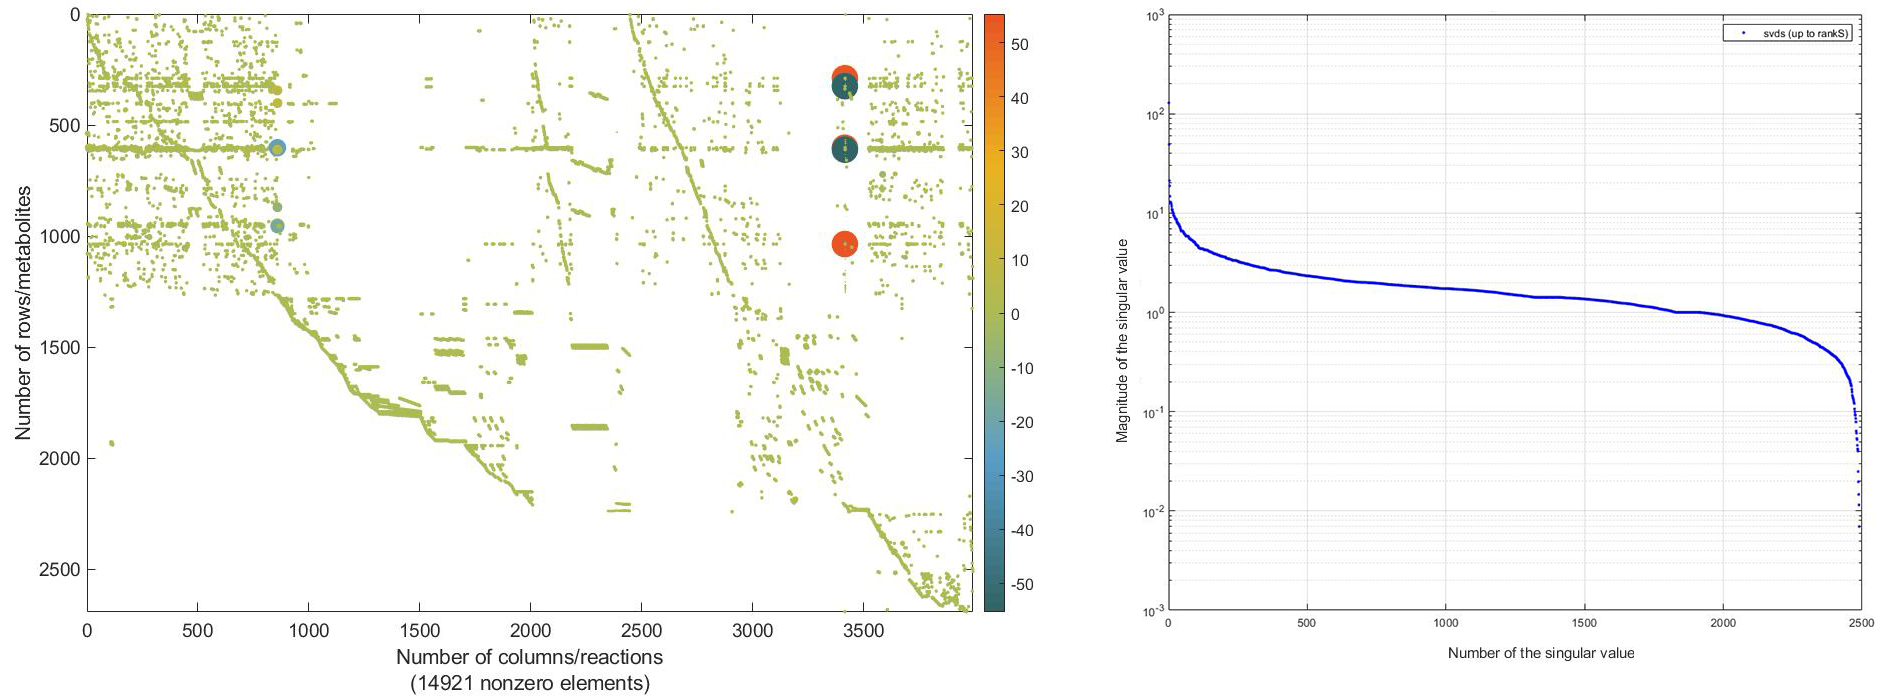
\includegraphics[width=1\columnwidth]{modelstats.png}
\end{center}
\caption[Coefficients and singular values of the stoichiometric matrix of Yeast8]{Coefficients and singular values of the stoichiometric matrix of Yeast8}
\label{fig:modelstats}
\end{figure}

All simulations in this chapter are done using Yeast8 v8.3.4 model which is hosted in Github (https://github.com/SysBioChalmers/yeast-GEM).

\begin{figure}[H]
\begin{center}
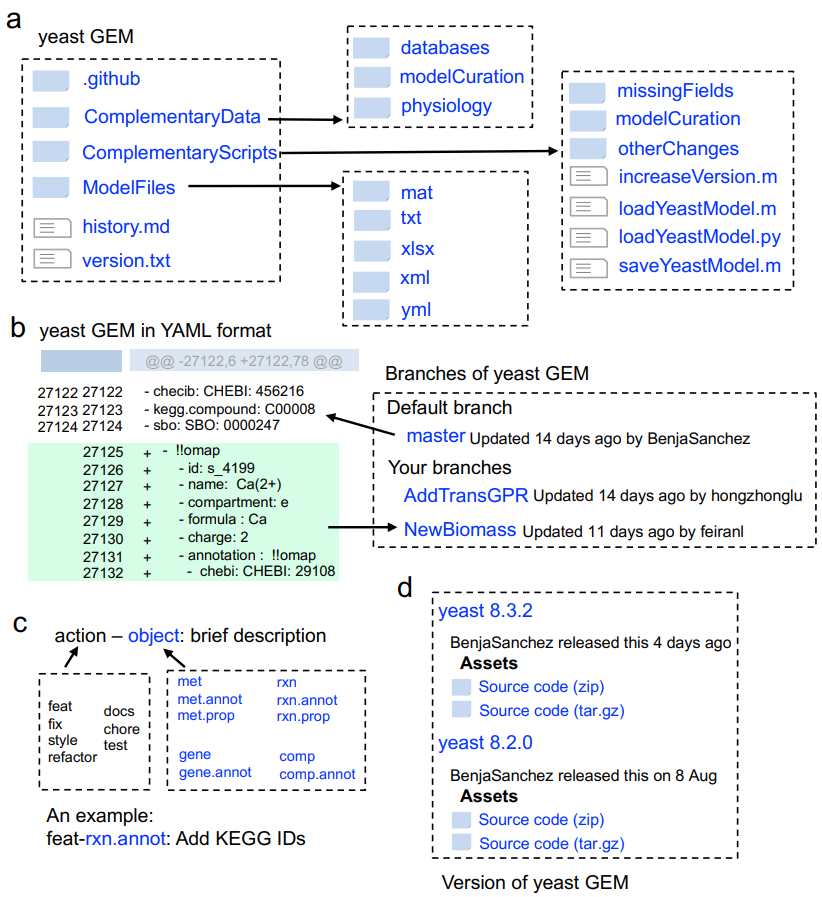
\includegraphics[width=0.9\columnwidth]{yeast8_github.png}
\end{center}
\caption[Repository of yeast GEM on GitHub]{Repository of yeast GEM on GitHub. Figure is taken from \cite{lu2019consensus}. ~ will be redrawned in thesis}
\label{fig:yeast8_github}
\end{figure}

\section{Chemostat Simulation: GAM Fitting}
In order to make sure the \emph{in-silico} obtained growth rate predictions are in agreement with the physiological kinetic parameters obtained from real experiments, fine adjustment on the energy reactions is a requirement. Since the growth-associated maintenance (GAM) and non-growth associated maintenance (NGAM) energy reactions play a determinant role in simulations, fluxes through these reactions must be constrained to a fixed value. Flux of NGAM is constrained to 0.7 mmol gDWh\textsuperscript{-1} for aerobic, and 0 mmol gDWh\textsuperscript{-1} for anaerobic simulations as calculated in the previous studies \cite{nilsson2016metabolic}. For the estimatation of GAM, since it depends on the biomass composition, findings of a chemostat experiment \cite{van1998effect} is used as a guide to fit predictions to. Model is simulated iteratively with a range of values for GAM, and the best fit is found at the level of 55.25 mmol gDWh\textsuperscript{-1} (Figure \ref{fig:Gam_fitting}), GAM flux is constrained accordingly.

\begin{figure}[H]
\begin{center}
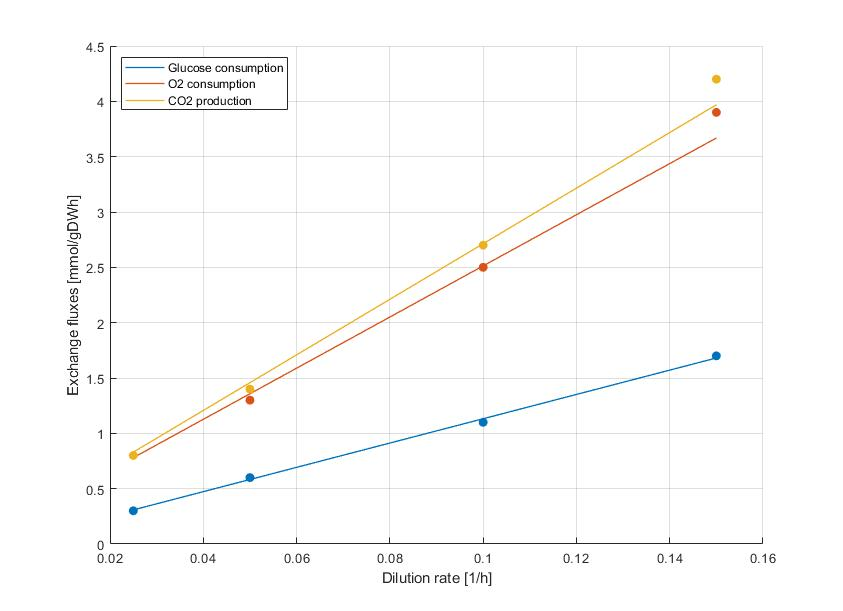
\includegraphics[width=0.8\columnwidth]{Gam_fitting.jpg}
\end{center}
\caption[Chemostat simulation to re-fit growth associated maintenance]{Chemostat simulation to re-fit growth associated maintenance.}
\label{fig:Gam_fitting}
\end{figure}

\section{Flux Balance Analysis}
Flux balance analysis (FBA) assumes that the living cells act as they optimized their lives towards some goal, and as if they were at steady state. To be more clear, steady-state assumption indicates that the metabolites are both produced and consumed at the same rate in a cell, without an accumulation. Therefore, in this system, metabolites are constrained by only the stoichiometric coefficients arised from mass balance of metabolites. As a result of this assumption, FBA solves a set of ordinary differential equations regarding to the stoichiometric matrix:
\begin{equation}
 \ S_{m \times n} \cdot v=0
\end{equation}
\noindent where S is the matrix of the stoichiometric reaction coefficients with m number of metabolites (as rows) and n number of reactions (as columns), and v is the vector of all associated reaction fluxes (mmol/gDWh). Because the matrix S usually has more reactions than metabolites (m<n), the system can result multiple solutions, and being called an underdetermined system. To solve it for an optimal solution, additional constraints are required.

A "growth reaction" is usually included in the reactions of the system to represent the "goal" in the definition of living systems. Growth reactions act as the final consumption of metabolites necessary for the biomass production or cell replication. Additional to the growth, several exchange reactions (uptake or secretion of metabolites from or into extracellular space) are also included. Since the concentrations of extracellular metabolites are measurable experimentall, constraints can be applied to exchange reaction fluxes to shrink solution space. The more constraints introduced into the system, such as reversibility of reactions or known rate values, result smaller solution space. The growth reaction is usually used as an objective function to determine a unique solution from this solution space. The linear problem appears as:
\begin{align}
 \ \text{max}_v \quad & c^T \cdot v \\
 \label{eq:fba}
 \ \text{subject to} \quad & S_{m \times n} \cdot v=0 \\
 \ & v_{lb} \leq v \leq v_{ub}
\end{align}
\noindent where c is the objective function vector, v is the vector of fluxes, S is the stoichiometric matrix as above equation. Subscripts lb and ub are the lower and upper boundaries on v. These constraints defines a feasible region of the problem.

In order to simulate batch conditions where minimal yeast medium is used, all the exchange reactions in the model are blocked first (lower bounds are set to 0). Then, only the exchange reactions of ions that are available to the cells in the experimental design (ammonium, phosphate, sulphate, iron(2+), H+, water, chloride, Mn\textsuperscript{2+}, Zn\textsuperscript{2+}, Mg\textsuperscript{2+}, sodium, Cu2\textsuperscript{2+}, Ca\textsuperscript{2+}, potassium) are set free (lower bounds are set to -1000), means that cells can uptake as it needs. While oxygen and glucose uptake rates decreased from 20 mmol gDWh\textsuperscript{-1} and increased to 20 mmol gDWh\textsuperscript{-1}, respectively, fluxes of ethanol, acetate, glycerol, formate, succinate secretion reactions with the growth rate is collected (Figure \ref{fig:fba}).
\hl{I need to show experimental results -preferably from the same article where I got expression data- on the figure to compare with my FBA results}

\begin{figure}[H]
\begin{center}
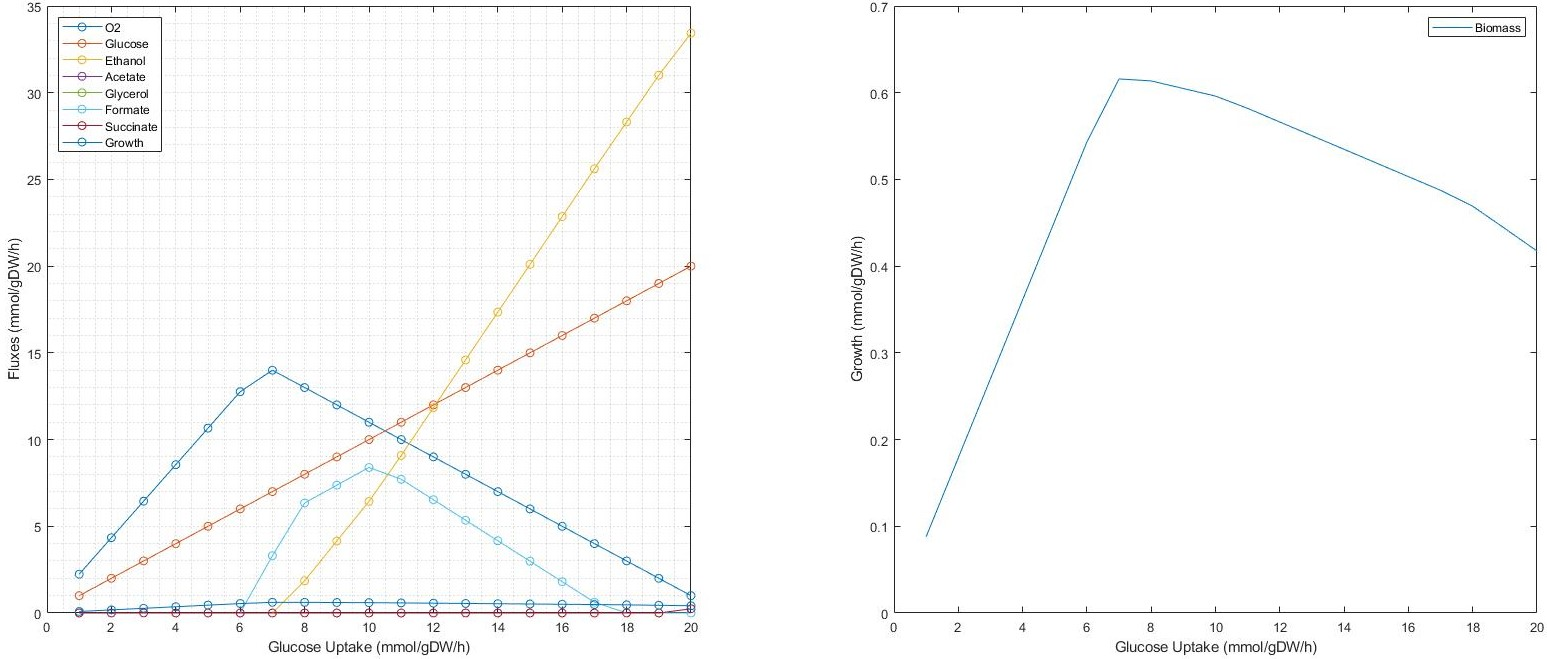
\includegraphics[width=1\columnwidth]{fba.jpg}
\end{center}
\caption[Flux balance simulation results]{Flux balance simulation results where oxygen uptake rate decreased and glucose uptake rate is increased simultaneously. Flux rates of several metabolites on the left, predicted growth rate on the right.}
\label{fig:fba}
\end{figure}

\section{Flux Variability Analysis}
Flux variability analysis (FVA) finds the minimum and maximum available fluxes for each reaction while obeying the provided constraints (for example fixed glucose uptake or growth rate). FVA is mainly used to evaluate the robustness of the model \cite{thiele2010functional}, to find alternative optimum states \cite{mahadevan2003effects}, to check flux distributions when growth is not at optimum level \cite{reed2004genome}, and it has many other applications \cite{gudmundsson2010computationally}.

FVA, similar to FBA, solves two optimization problems for each reaction:
 \begin{align}
 \ \text{max}_v / \text{min}_v \quad & v_i \\
 \ \text{subject to} \quad & S_{m \times n} \cdot v=0 \\
 \ & w^T \cdot v \geq \gamma \cdot Z_0 \\
 \ & v_{lb} \leq v \leq v_{ub}
 \end{align}
\noindent where $w$ is the objective function equals to $c$ in the problem \ref{eq:fba}, $Z_0 = w^T \cdot v_0$ describes an optimal solution to the problem \ref{eq:fba}, $\gamma$ is an indicator to check whether the FVA is done at the optimal state (where objective flux is the same and $\gamma = 1$) or any other state (where $0 \leq \gamma < 1$).

Flux variabilites of Yeast8 reactions are analyzed by solving the linear problem with the objective functions to minimize and maximize all reactions iteratively with tolerance value of 1e-9 using the GUROBI solver. Minimum and maximum available fluxes are collected in the iterative process for each reaction, and results are plotted for glycolysis, pentose phosphate pathway and TCA pathway reactions as error boxes (Figure \ref{fig:fva}). Flux values obtained through the ordinary FBA solution are also shown as a line.

\begin{figure}[H]
\begin{center}
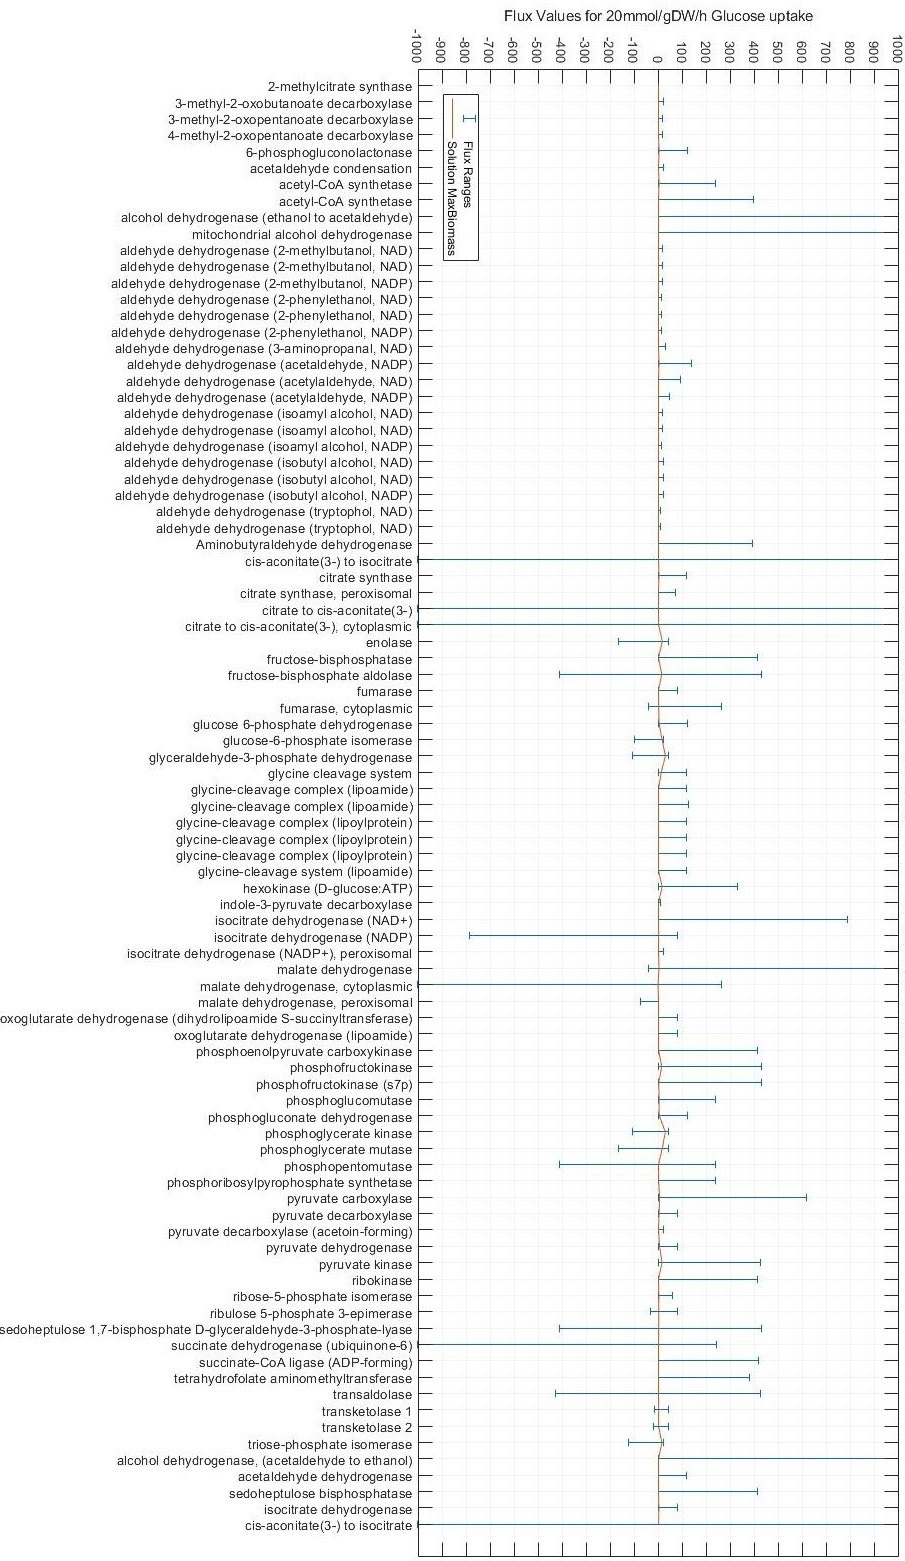
\includegraphics[width=0.8\columnwidth]{fva_ranges.jpg}
\end{center}
\caption[Minimum and maximum fluxes of Glycolysis, PPP and TCA reactions]{Minimum and maximum fluxes of Glycolysis, PPP and TCA reactions.}
\label{fig:fva}
\end{figure}

\section{Phenotype Phase Plane Construction}

As mentioned in the FBA and FVA sections, there is no single solution to the linear problem of the model. Phenotype phase planes (PhPP) are used to describe all feasible metabolic states in a two or three dimentional surfaces, depending on the number of metabolites chosen to see how they affect the objective function \cite{edwards2002characterizing}. In general, for aerobic models, various levels of glucose and oxygen availability through their uptake reactions are used to generate PhPP surfaces in three dimention with objective function. Fundamentally, PhPP construction refers to a double robustness analysis on the model for selected reactions.

\begin{figure}[H]
\begin{center}
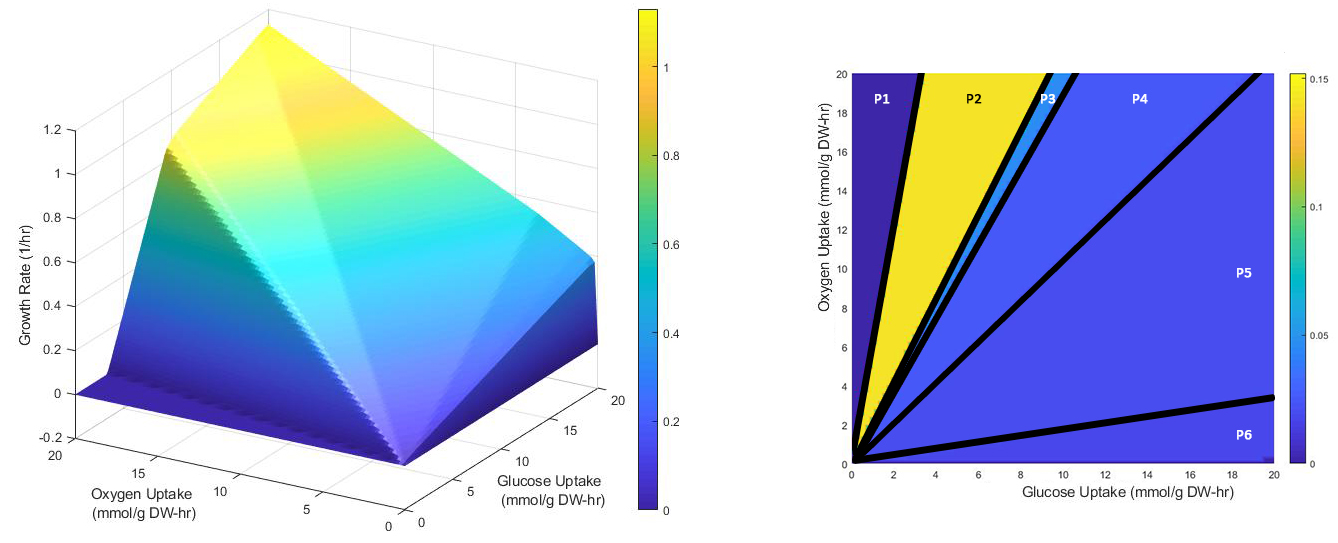
\includegraphics[width=1\columnwidth]{phpp.jpg}
\end{center}
\caption[Phenotype Phase Plane of Yeast8]{Phenotype Phase Plane of Yeast8, corresponding to glucose and oxygen availabilities on the left. Shadow prices of glucose on the right.}
\label{fig:phpp}
\end{figure}

\hl{In the results section of this, FBA simulations will be discussed with the phases observed in PhPP.}


\section{Random Sampling of Solution Space}
Constraints applied to a model define a solution space, a convex polytope, where every flux distribution is accessible. Random sampling of the solution space is an unbiased tool to explore metabolic models. Mainly, Markov Chain Monte Carlo methods are used to sample this space using algorithms such as (Artificially Centered) Hit-and-Run (HRB) \cite{kiatsupaibul2011analysis, saa2016ll} algorithm, and this method has proven to be helpful in the analysis of genome-scale metabolic models \cite{schellenberger2009use}. Briefly, the random sampling method collects points that are uniformly distributed in the solution space and calculates the most probable flux value for each reaction.

\begin{figure}[H]
\begin{center}
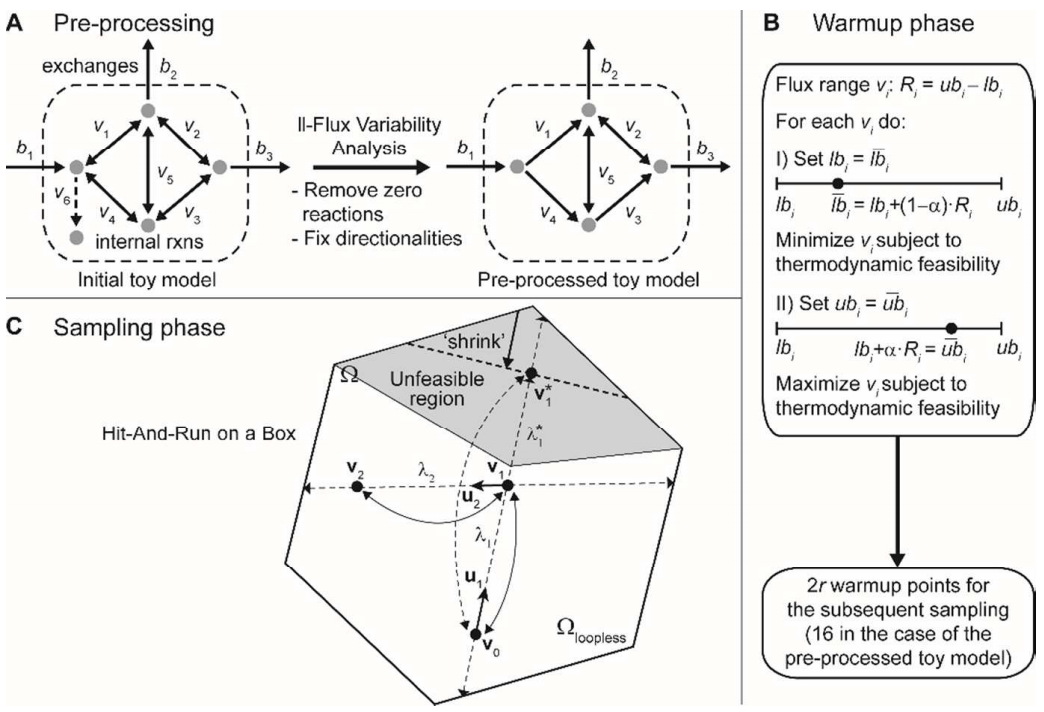
\includegraphics[width=1\columnwidth]{ll-achrb.png}
\end{center}
\caption[Workflow of the Loopless-ACHRB sampling on a toy model]{Workflow of the ll-ACHRB sampling on a toy model. A) Pre-processing phase, application of loopless-FBA to remove blocked reactions and constraining the directionalities of others. B) Warmup phase, modifying the reaction bounds to more interior space. C) Sampling phase with HRB algorithm. Figure is taken from \cite{saa2016ll}}
\label{fig:achrb}
\end{figure}

Since the computational burden of loopless sampling is high, generated random points in the solution space of Yeast8 includes thermodynamically unfeasble states. Maximum glucose uptake rate was constrained to 1 mmol gDWh\textsuperscript{-1} and total of 5000 points are generated with maximum of 120 secondse alloted for the sampling.

\begin{figure}[H]
\begin{center}
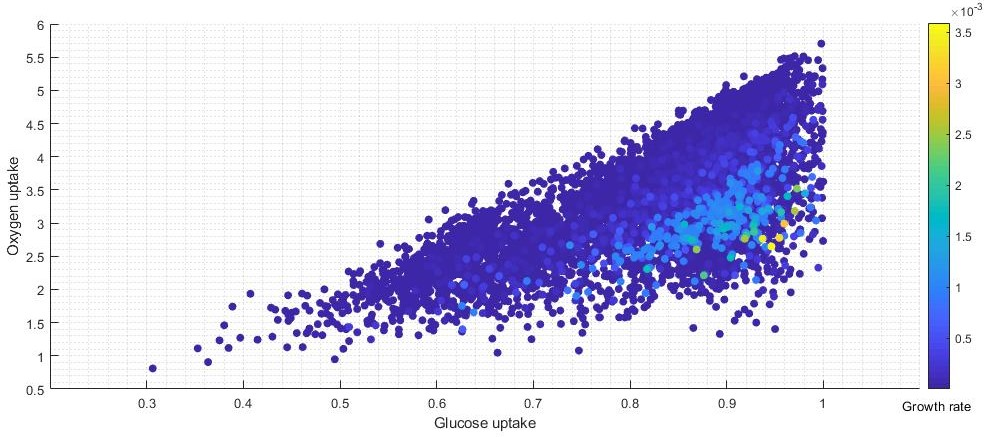
\includegraphics[width=1\columnwidth]{sampling_scatter_gluo2.jpg}
\end{center}
\caption[Scatter plot of glucose and oxygen uptake points from sampling]{Scatter plot of glucose and oxygen uptake points from sampling regarding growth rate.}
\label{fig:sampling_scatter_gluo2}
\end{figure}

\hl{From this point, there are only plots or resulted tables (all results will be put into "results" section later. They are in methods for simplicity.)}


\begin{landscape}
 \begin{figure}[H]
    \begin{sidewaysfigure}
     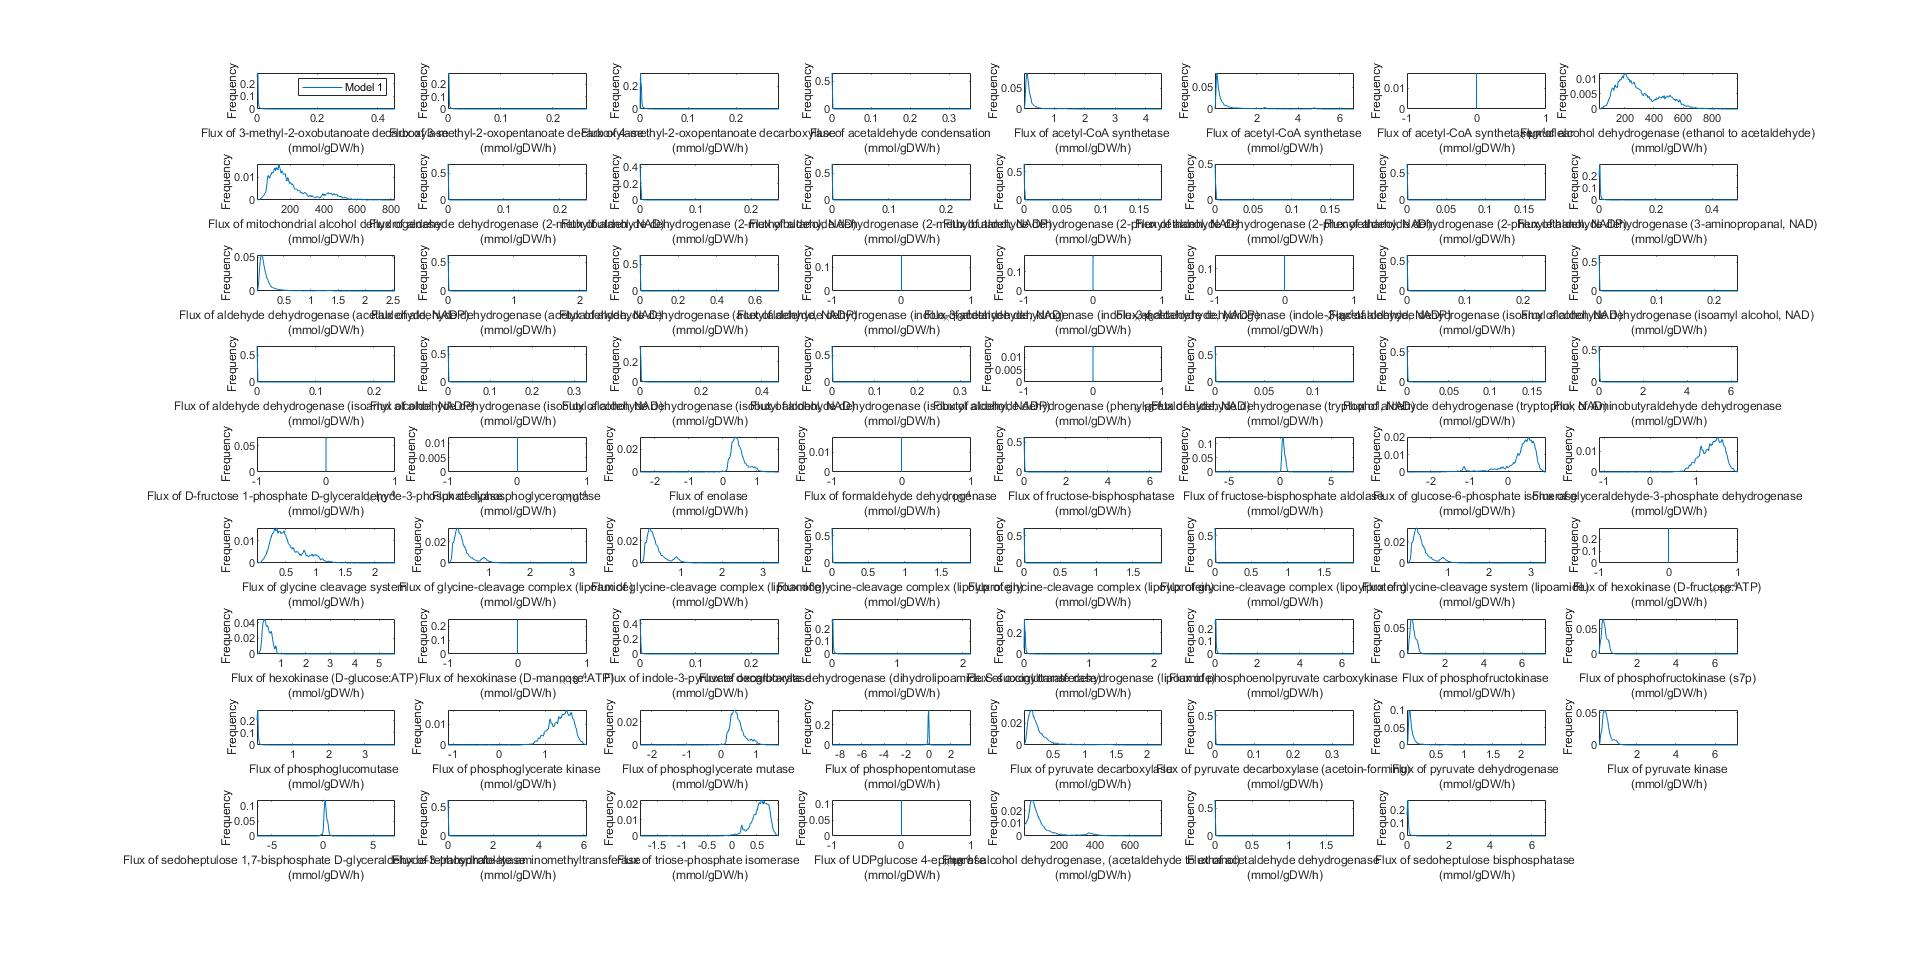
\includegraphics[width=1\columnwidth]{sampling_Hist_Glycolysis.jpg}
    \end{sidewaysfigure}
 \caption[Histogram plots of available flux values for glycolysis reactions]{Histogram plot of sampled points in glycolysis reactions.}
 \label{fig:sampling_Hist_Glycolysis}
 \end{figure}

 \begin{figure}[H]
    \begin{sidewaysfigure}
     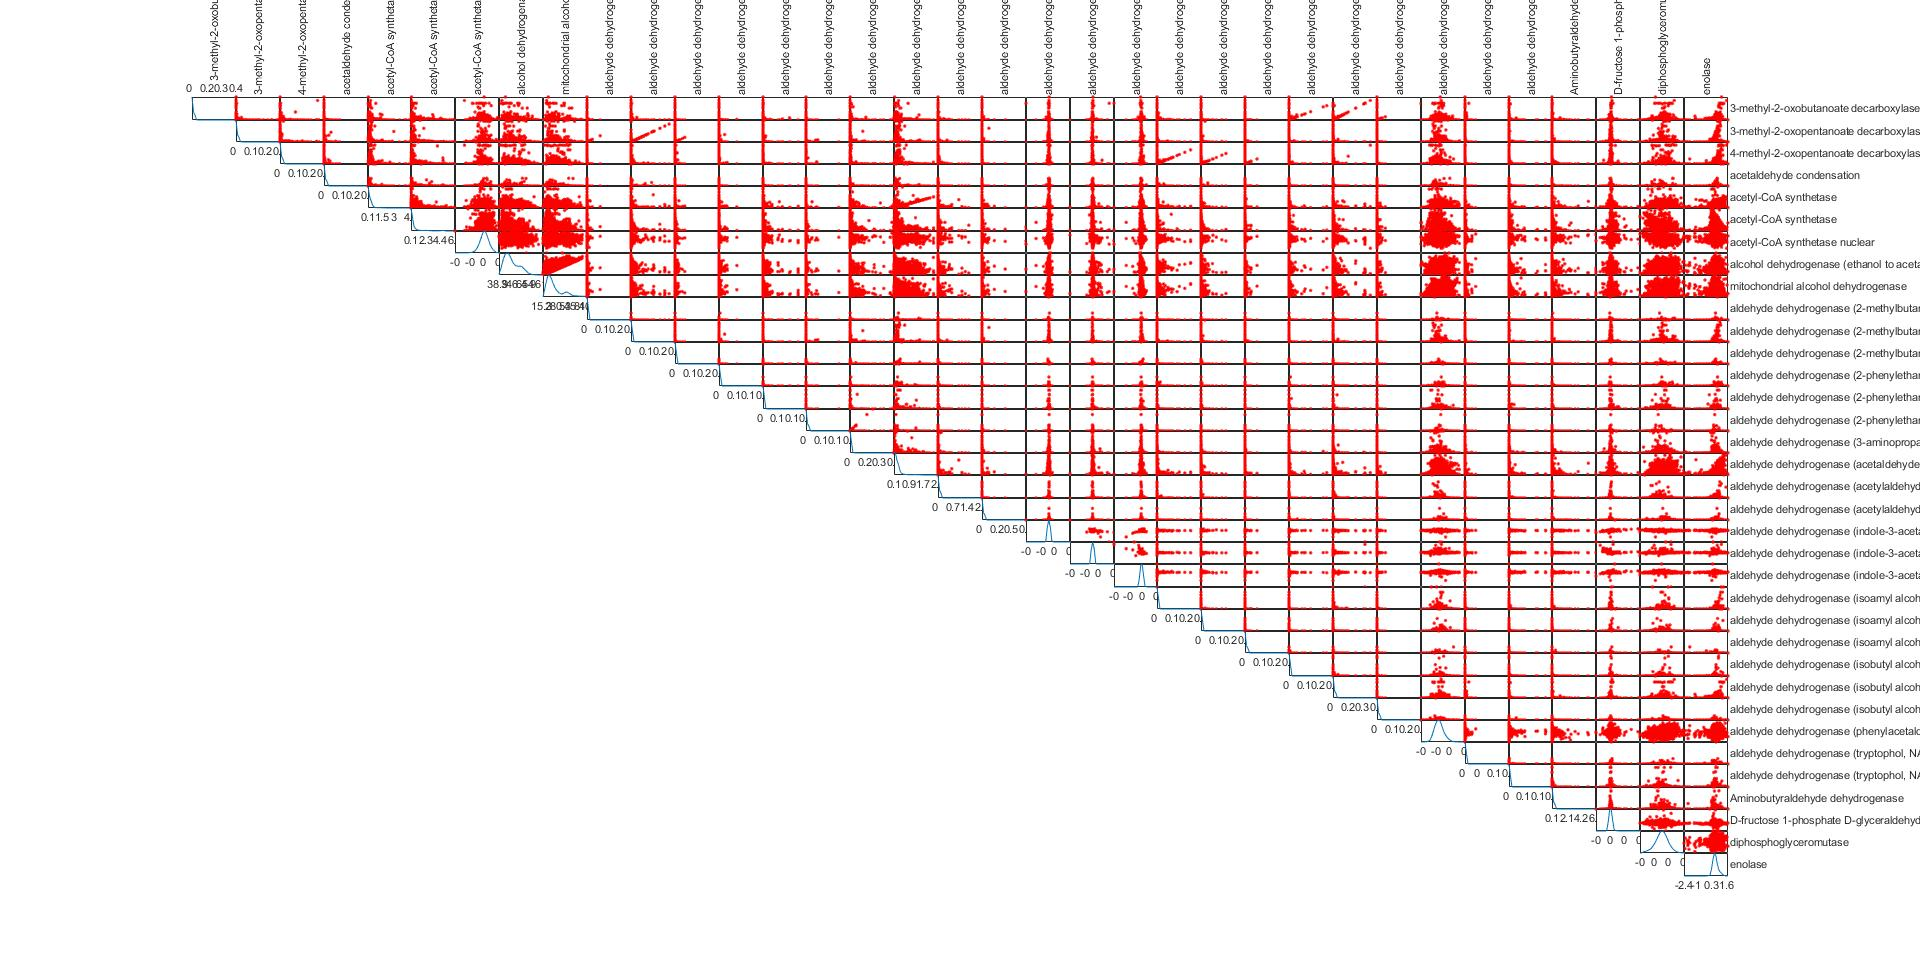
\includegraphics[width=1\columnwidth]{sampling_Scatter_Glycolysis_1.jpg}
    \end{sidewaysfigure}
 \caption[Correlations in between glycolysis reactions]{Correlations in between glycolysis reactions.}
 \label{fig:sampling_Scatter_Glycolysis_1}
 \end{figure}

 \begin{figure}[H]
   \begin{sidewaysfigure}
    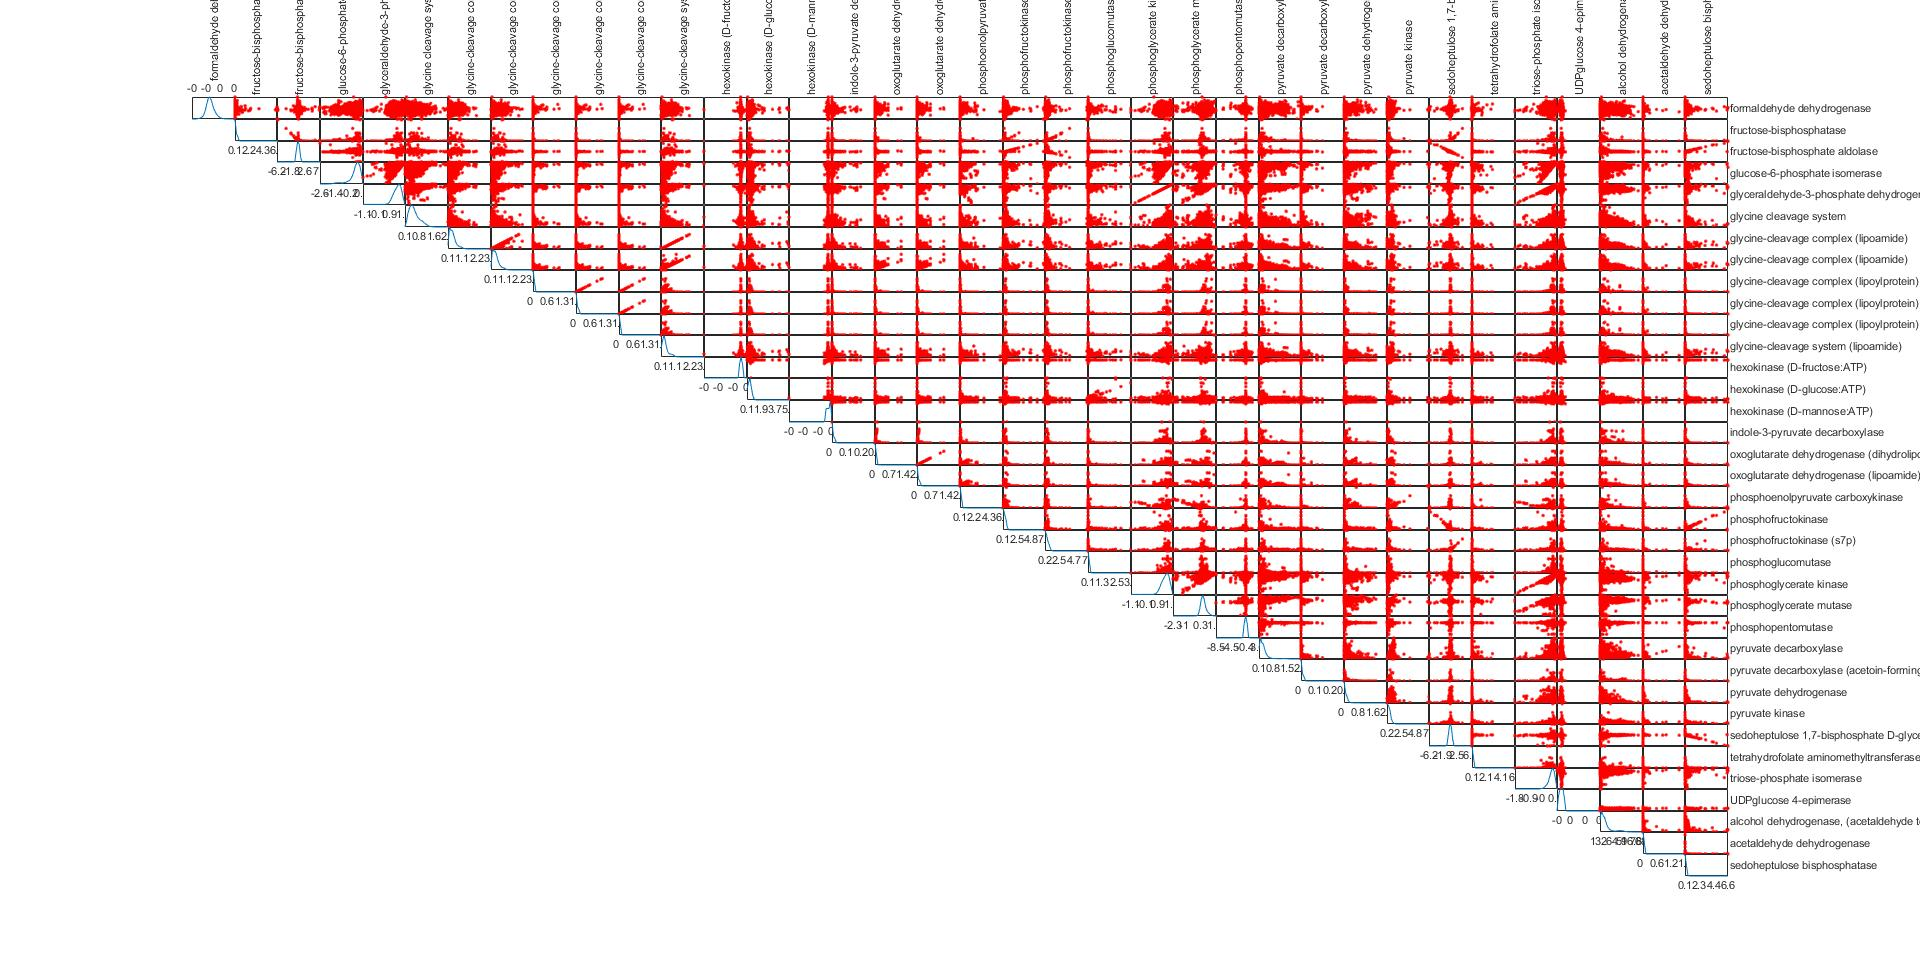
\includegraphics[width=1\columnwidth]{sampling_Scatter_Glycolysis_2.jpg}
    \end{sidewaysfigure}
 \caption[Correlations in between glycolysis reactions, continued]{Correlations in between glycolysis reactions, continued.}
 \label{fig:sampling_Scatter_Glycolysis_2}
 \end{figure}

  \begin{figure}[H]
     \begin{sidewaysfigure}
      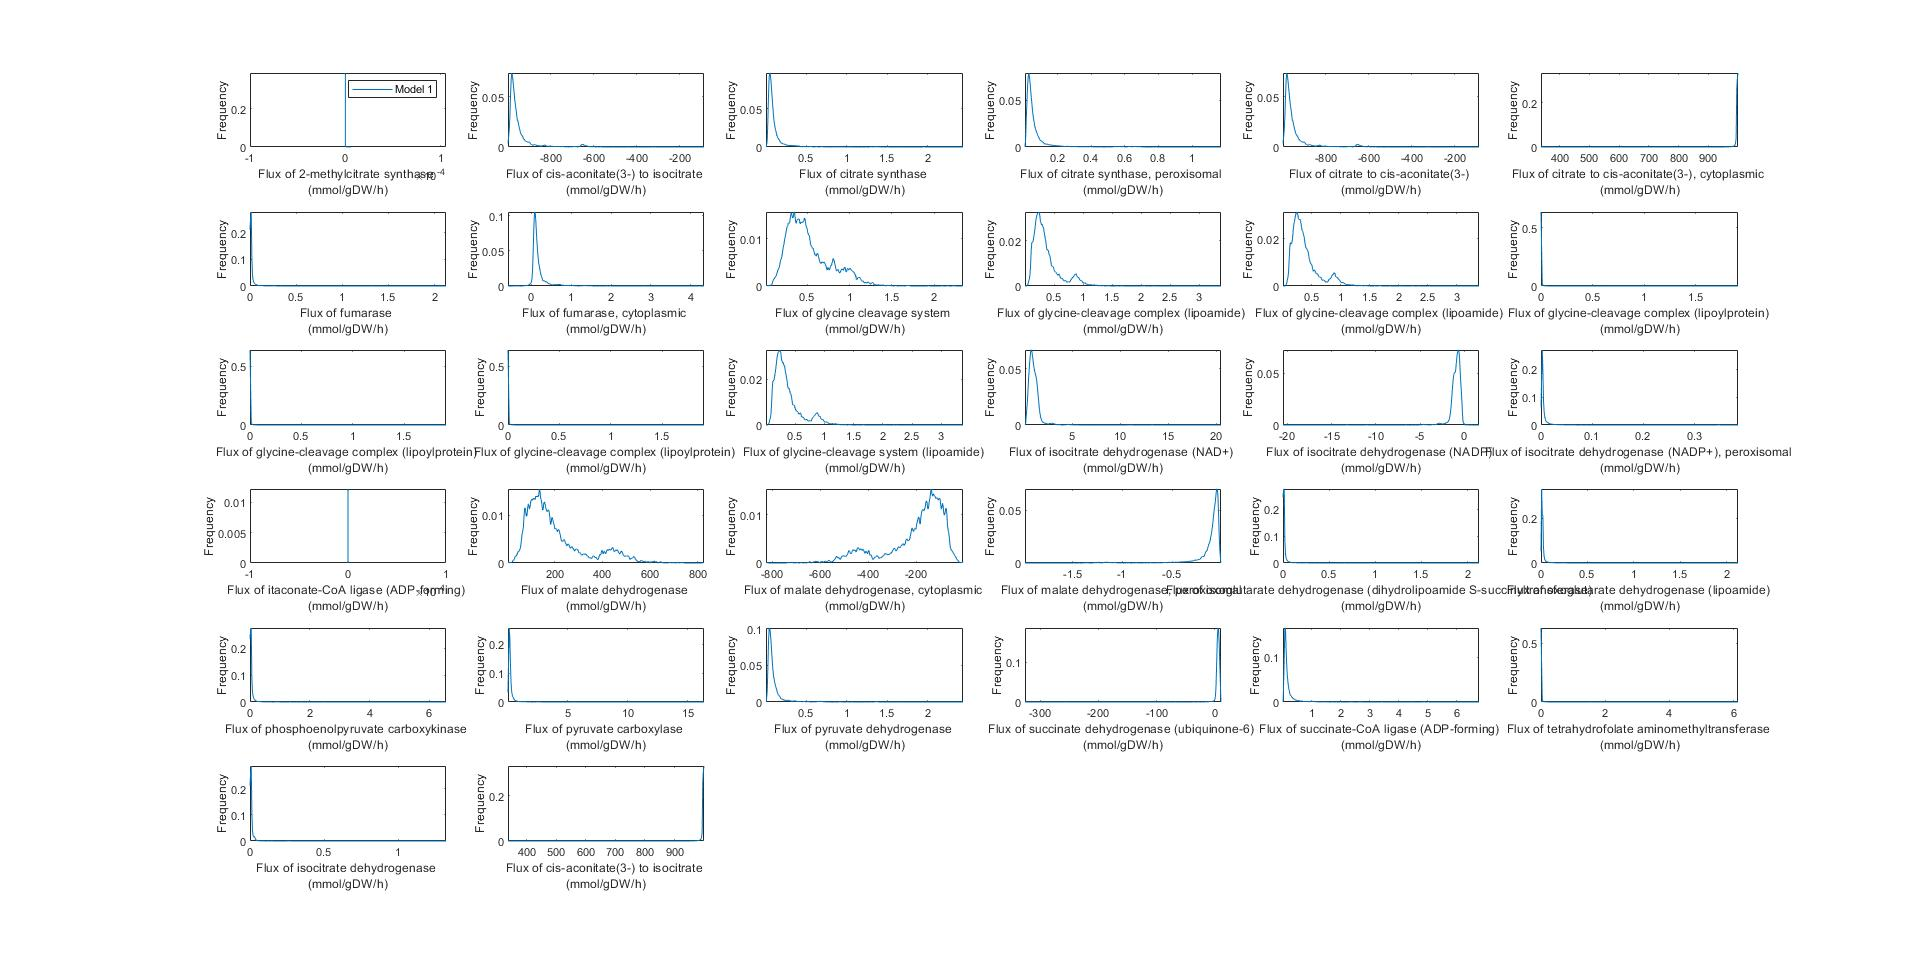
\includegraphics[width=1\columnwidth]{sampling_Hist_TCA.jpg}
     \end{sidewaysfigure}
  \caption[Histogram plots of available flux values for TCA reactions]{Histogram plot of sampled points in TCA reactions.}
  \label{fig:sampling_Hist_TCA}
  \end{figure}

  \begin{figure}[H]
   \begin{center}
     \begin{sidewaysfigure}
      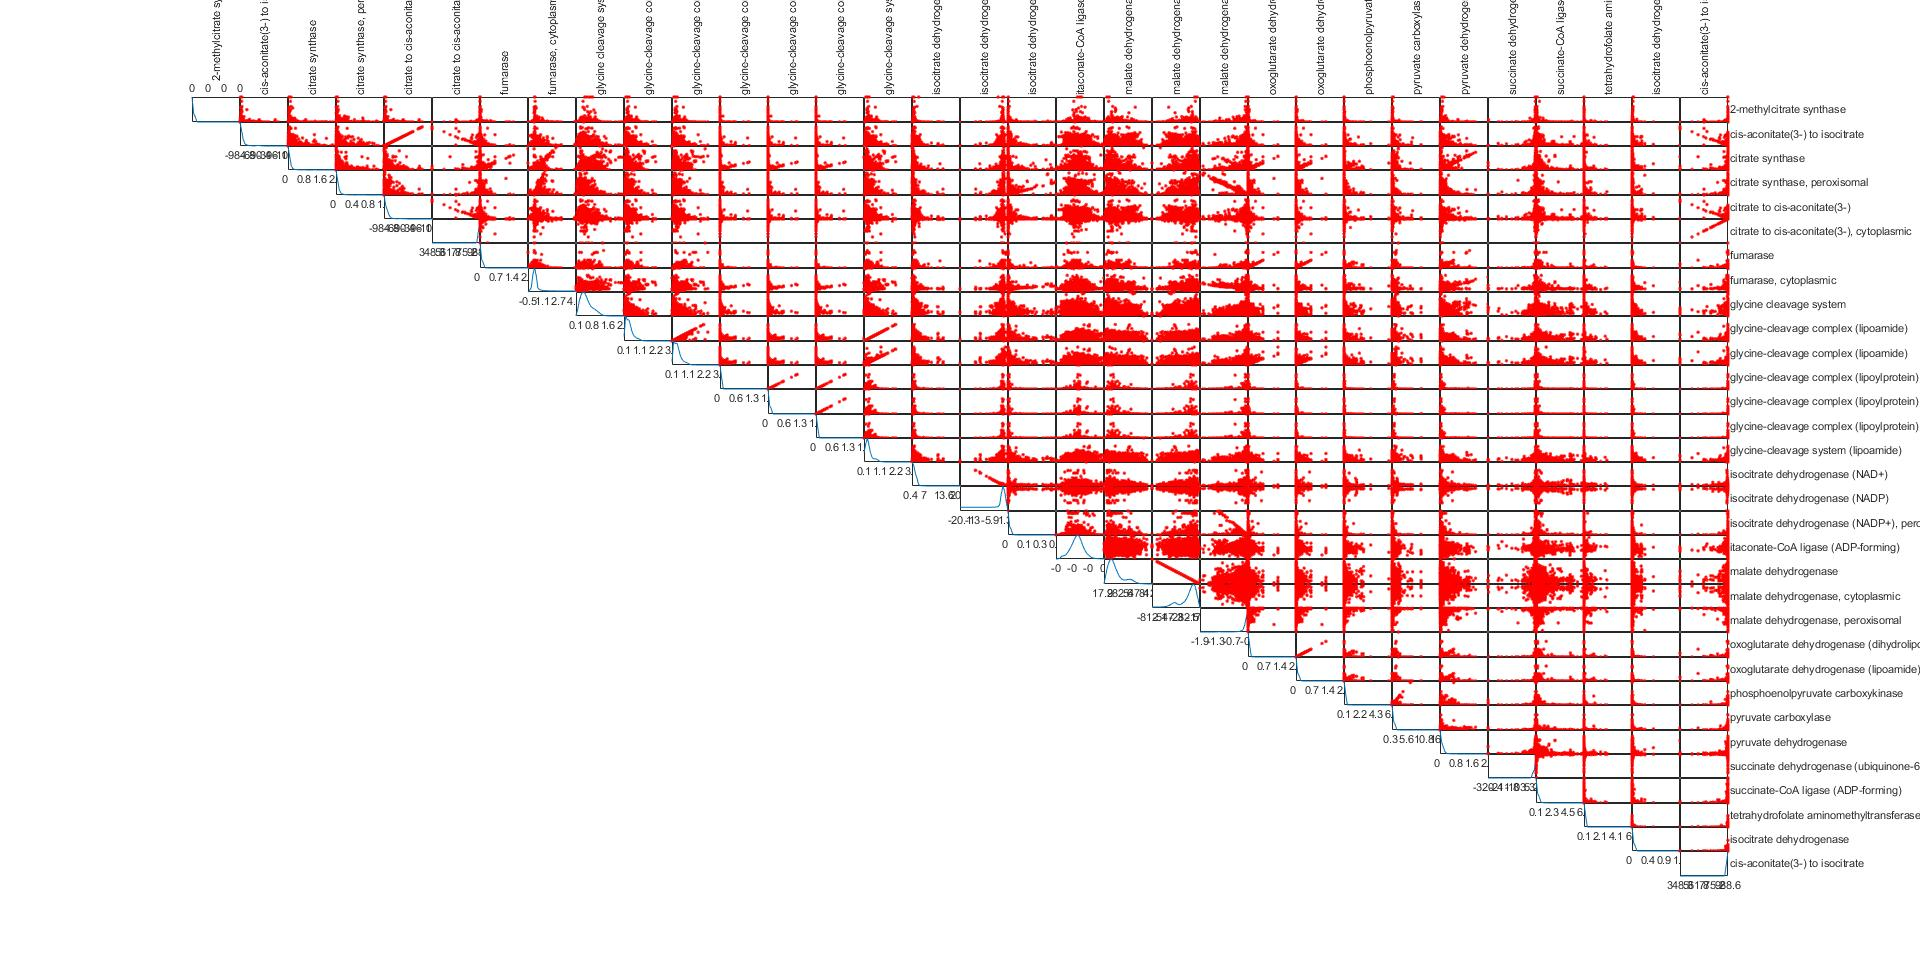
\includegraphics[width=1\columnwidth]{sampling_Scatter_TCA.jpg}
     \end{sidewaysfigure}
   \end{center}
  \caption[Correlations in between TCA reactions]{Correlations in between TCA reactions}
  \label{fig:sampling_Scatter_TCA}
  \end{figure}

   \begin{figure}[H]
    \begin{center}
      \begin{sidewaysfigure}
       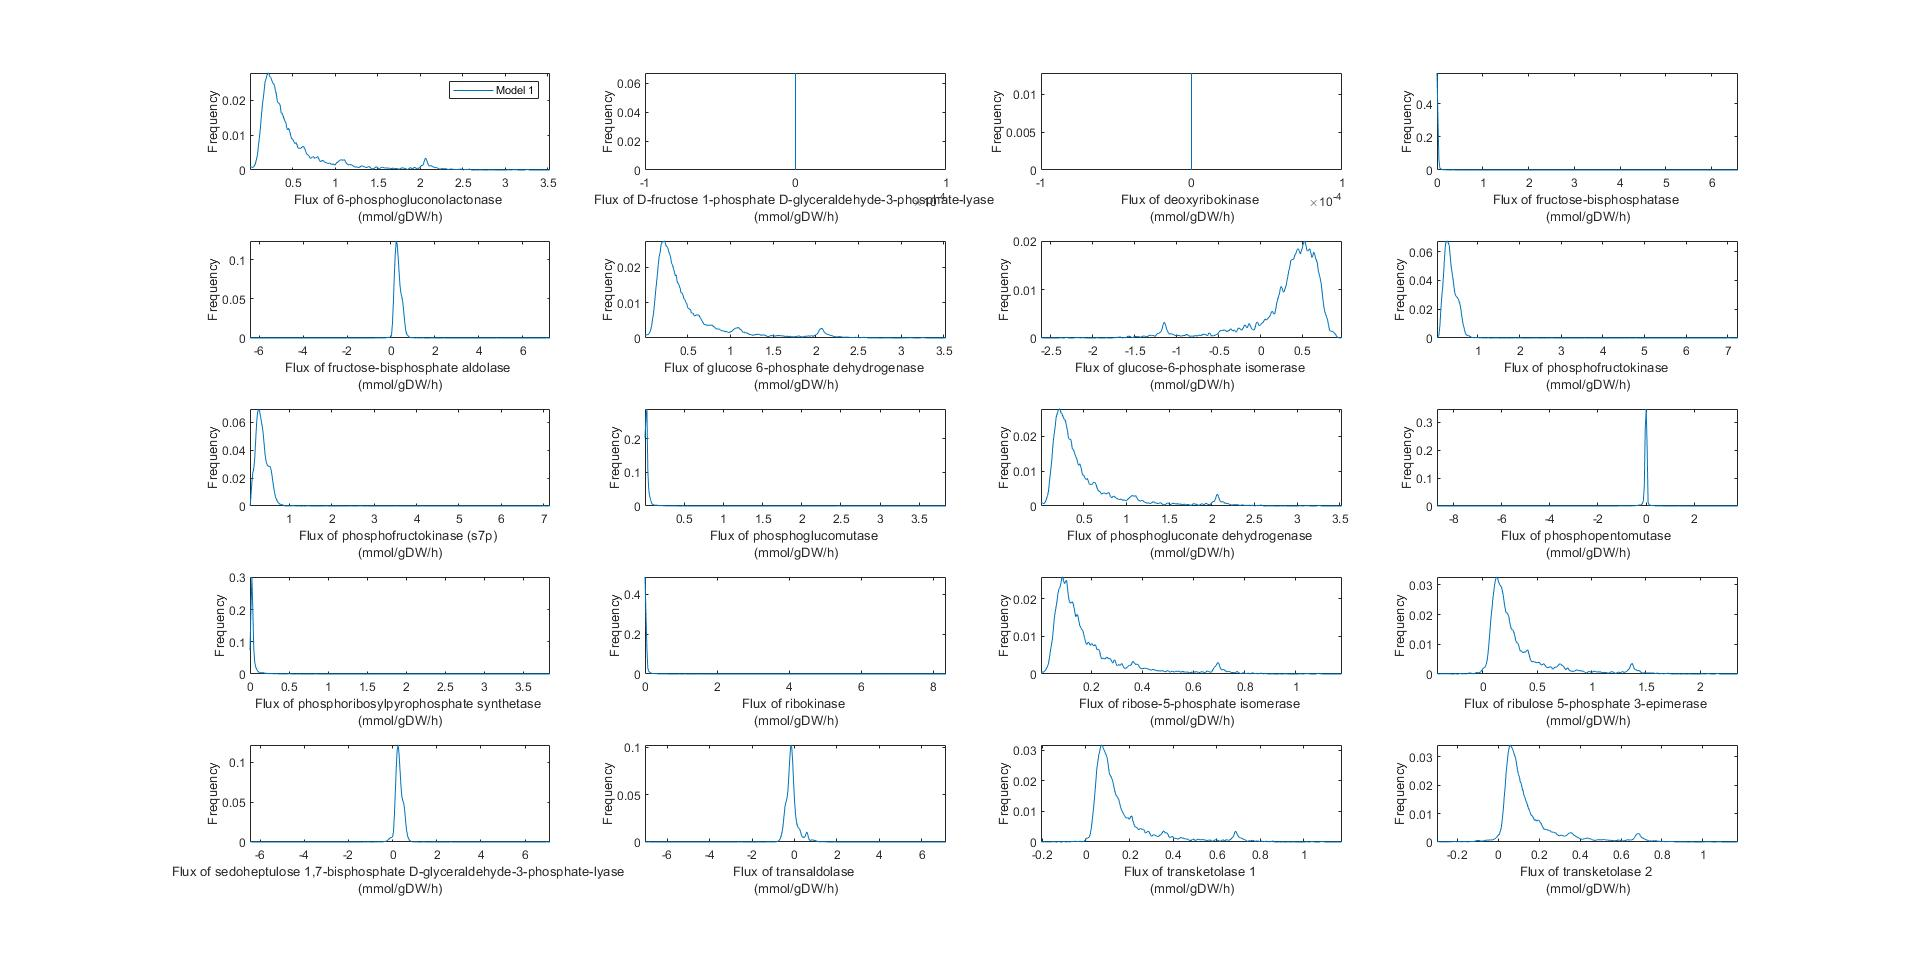
\includegraphics[width=1\columnwidth]{sampling_Hist_PPP.jpg}
      \end{sidewaysfigure}
    \end{center}
   \caption[Histogram plots of available flux values for PPP reactions]{Histogram plot of sampled points in PPP reactions.}
   \label{fig:sampling_Hist_PPP}
   \end{figure}

   \begin{figure}[H]
    \begin{center}
      \begin{sidewaysfigure}
       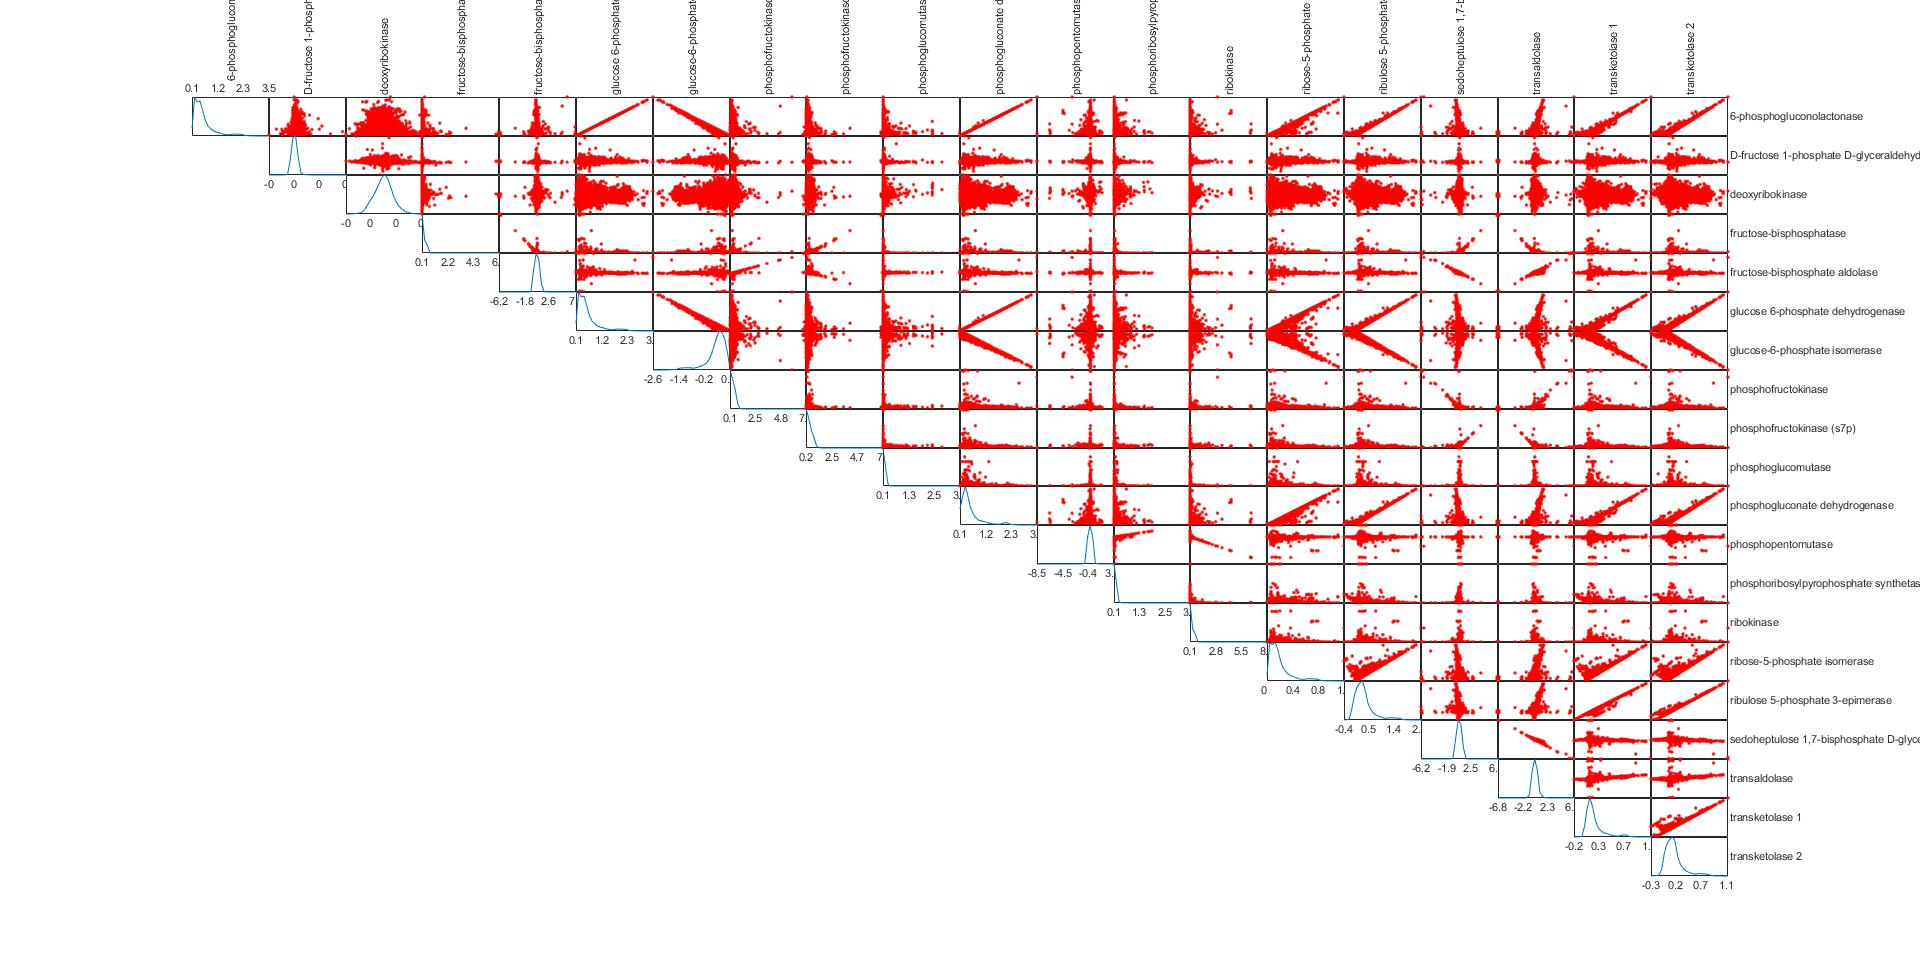
\includegraphics[width=1\columnwidth]{sampling_Scatter_PPP.jpg}
      \end{sidewaysfigure}
    \end{center}
   \caption[Correlations in between PPP reactions]{Correlations in between PPP reactions}
   \label{fig:sampling_Scatter_PPP}
   \end{figure}
\end{landscape}


\section{Knocking Out Single Genes and Reactions}

\begin{figure}[H]
\begin{center}
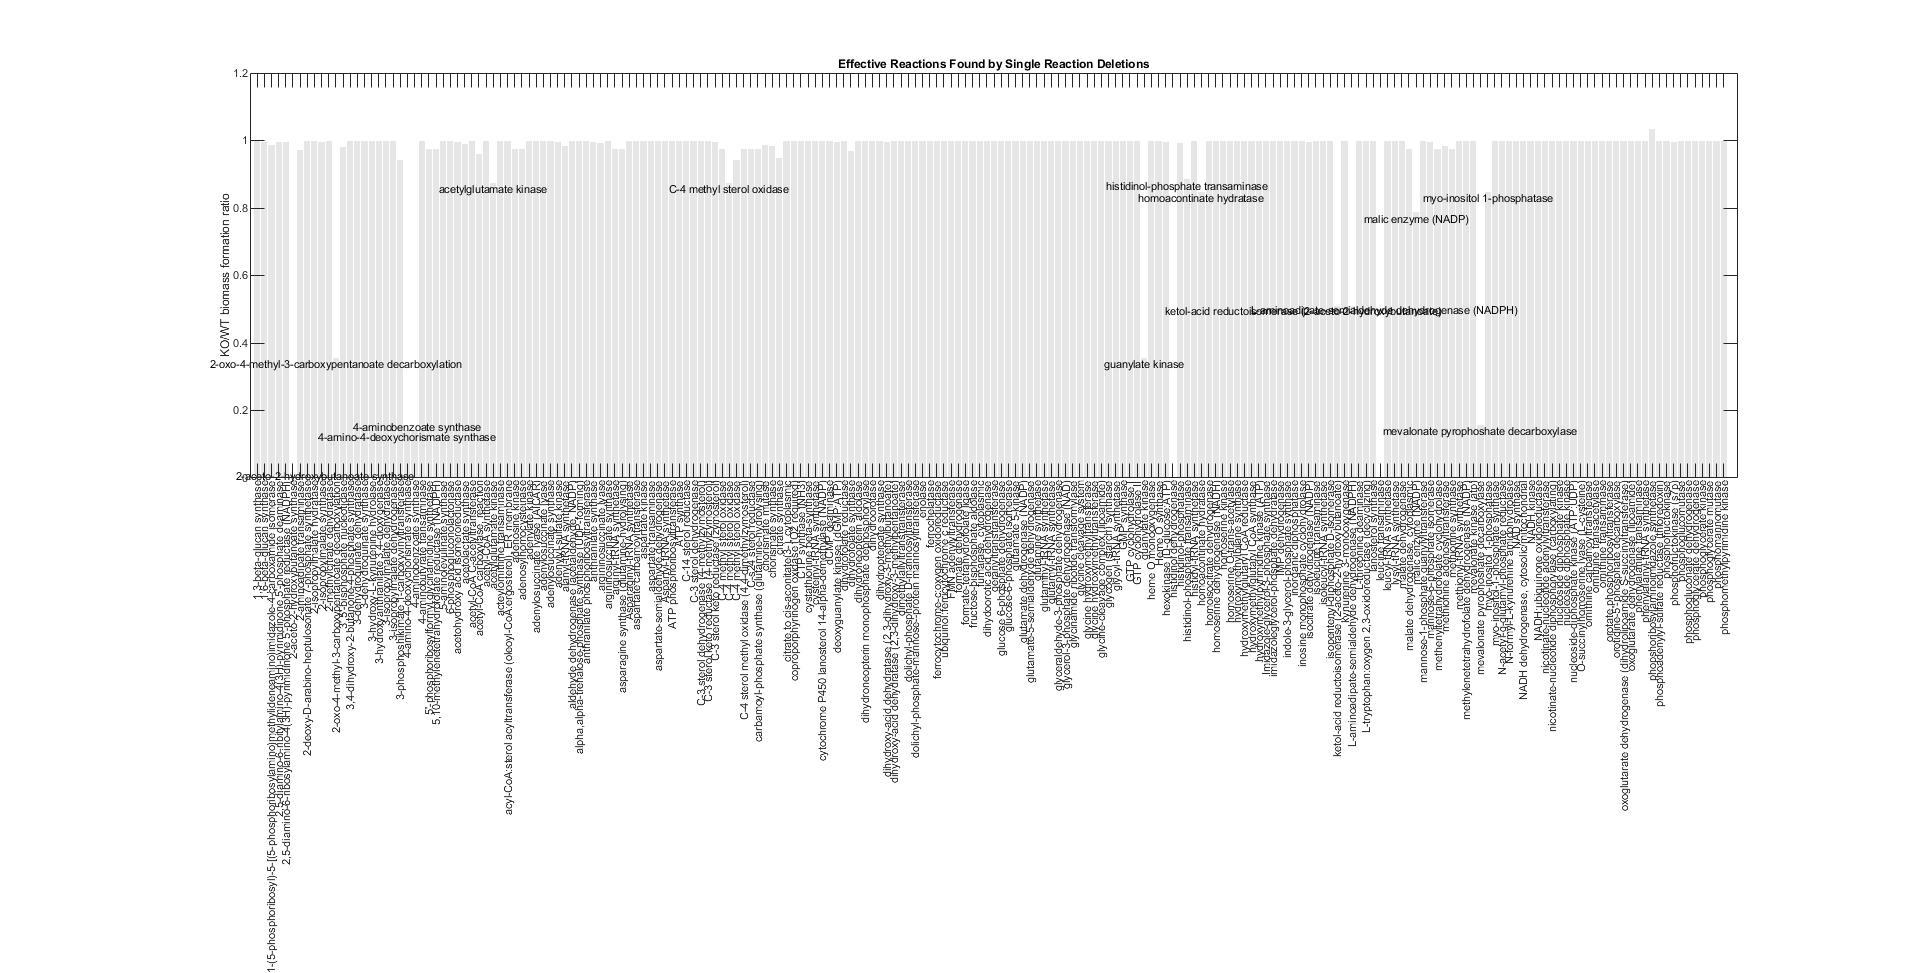
\includegraphics[width=1\columnwidth]{srd_fba.jpg}
\end{center}
\caption[Effective reactions found from the deletion analysis using FBA]{Effective reactions (not entirely essential, but  their absence changes the flux distribution or value of the optimization function) obtained from single reaction deletion simulations using FBA and their effect on growth rate is plotted.}
\label{fig:srd_fba}
\end{figure}

\begin{figure}[H]
\begin{center}
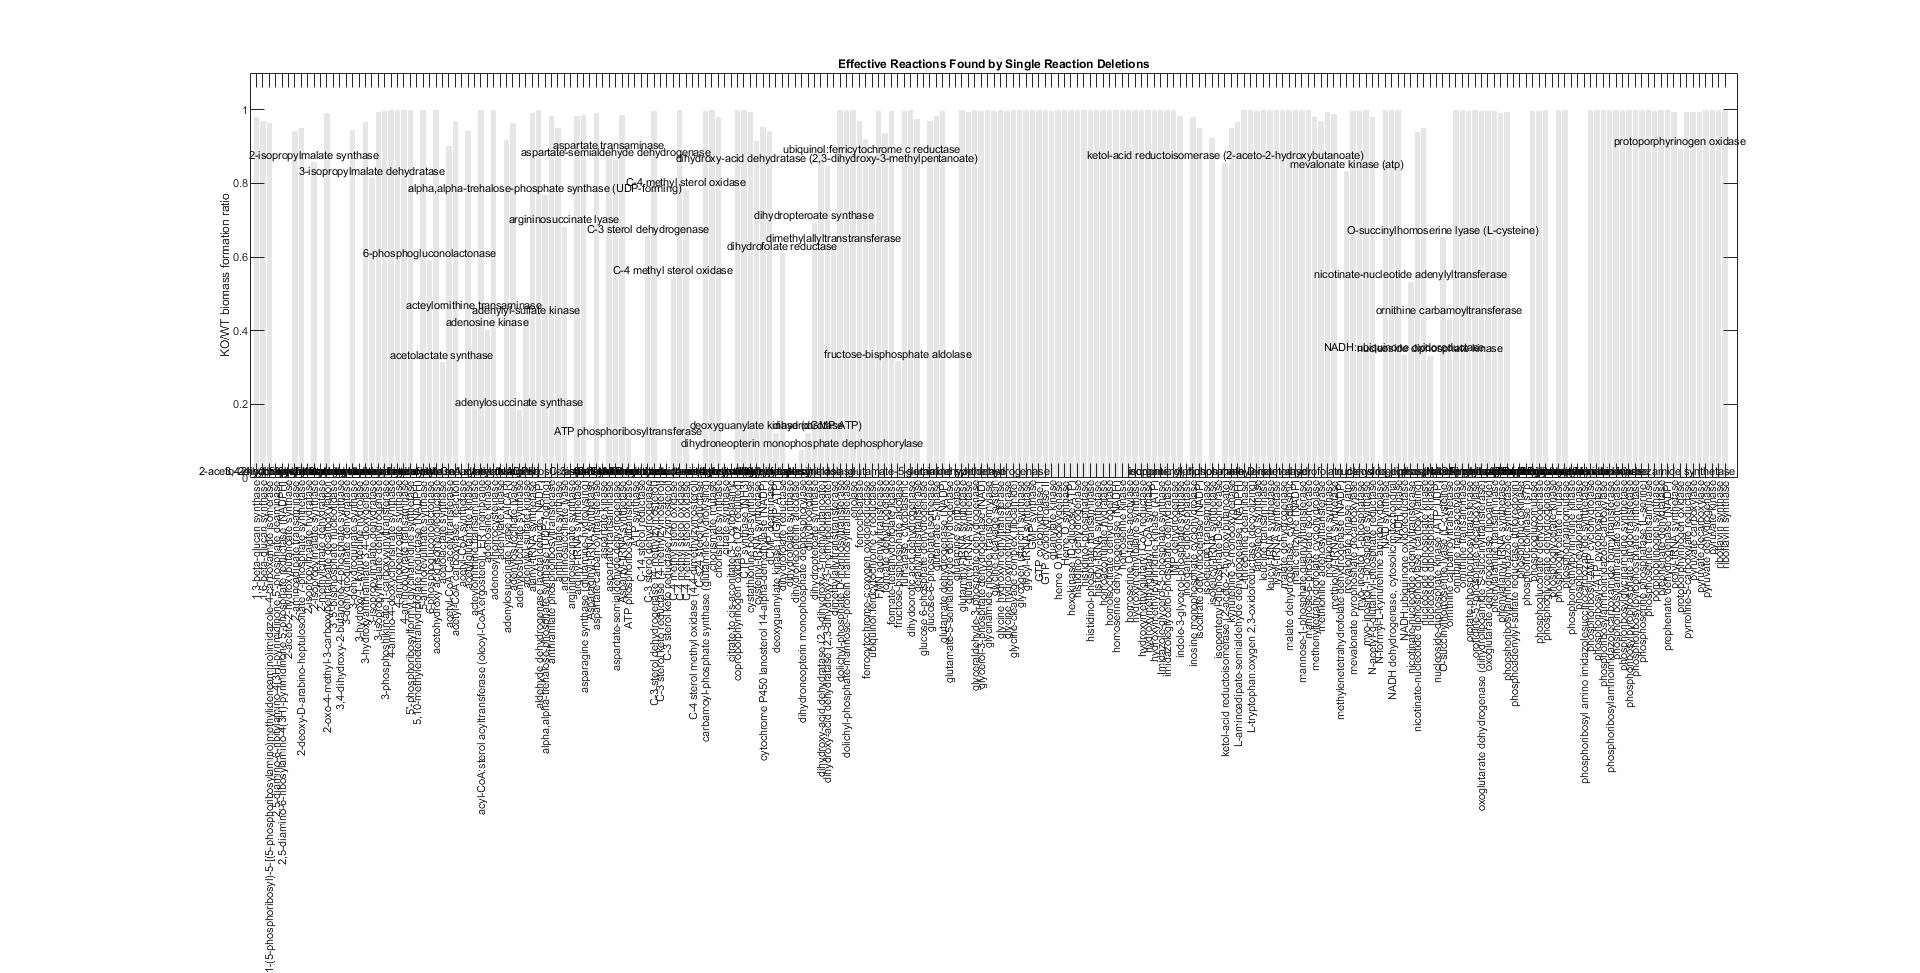
\includegraphics[width=1\columnwidth]{srd_moma.jpg}
\end{center}
\caption[Effective reactions found from the deletion analysis using MOMA]{Effective reactions (not entirely essential, but  their absence changes the flux distribution or value of the optimization function) obtained from single reaction deletion simulations using MOMA and their effect on growth rate is plotted.}
\label{fig:srd_moma}
\end{figure}


\begin{figure}[H]
\begin{center}
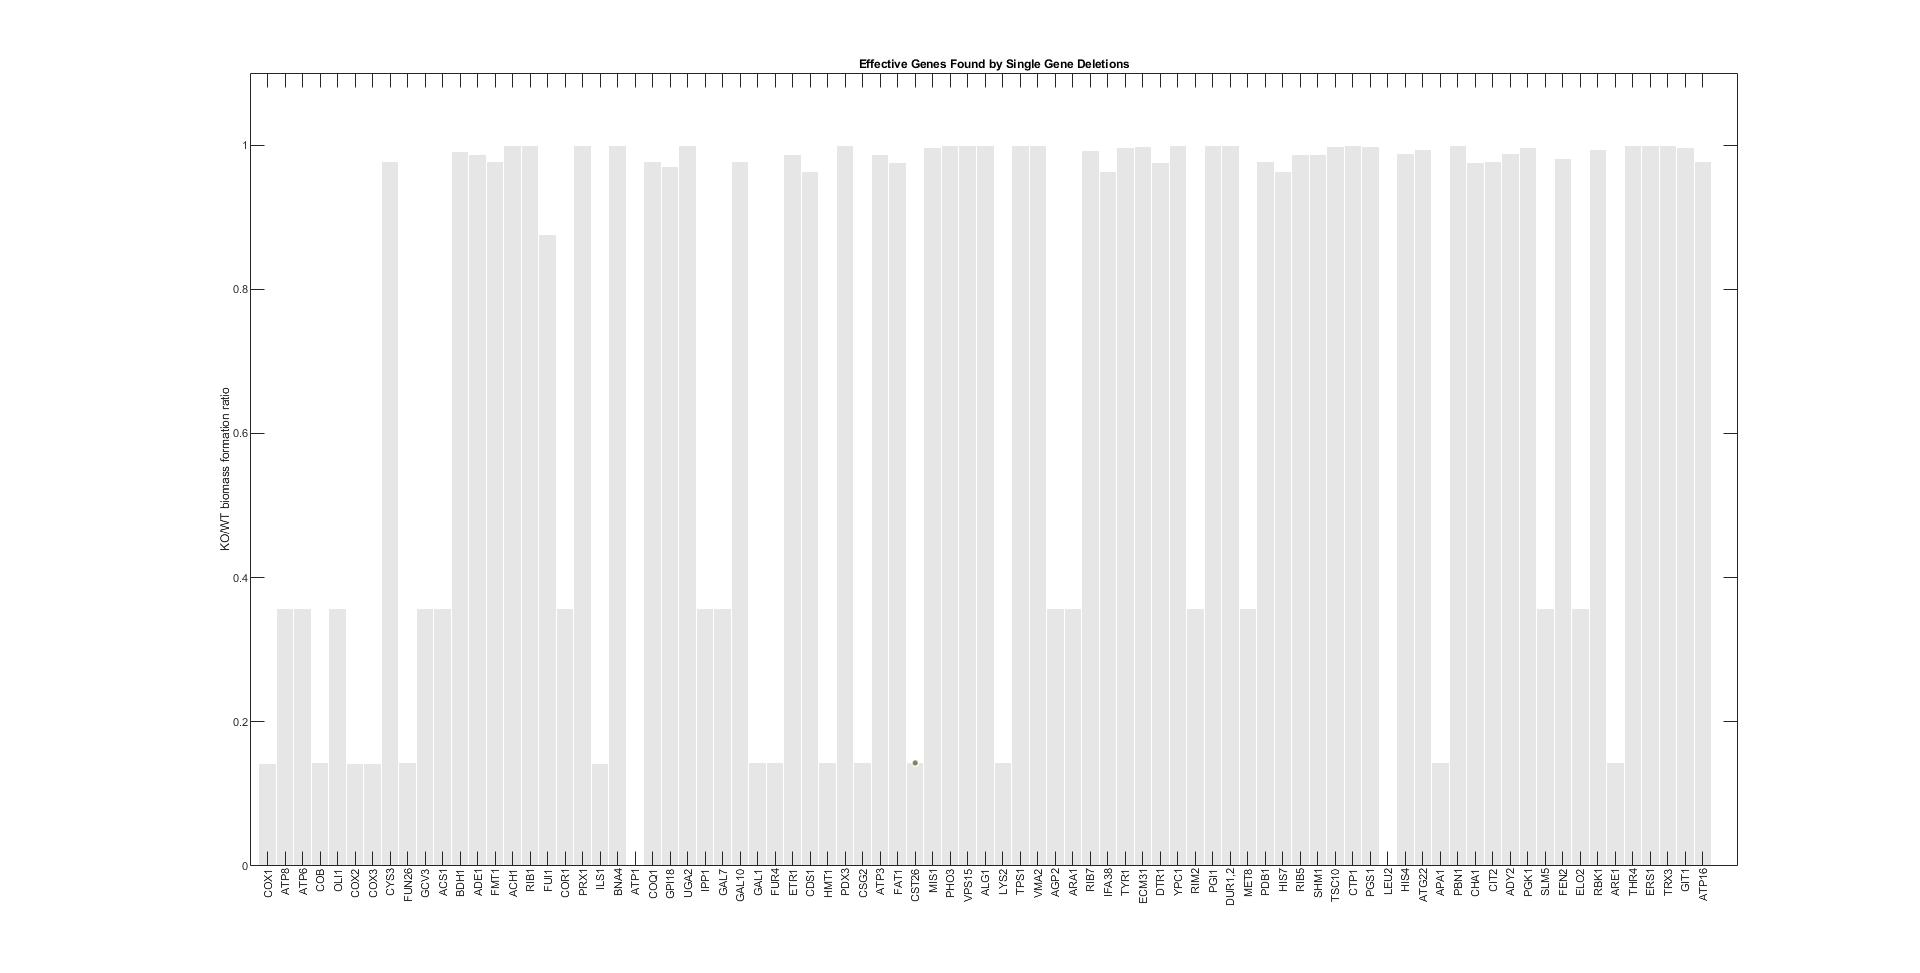
\includegraphics[width=1\columnwidth]{sgd_fba.jpg}
\end{center}
\caption[Effective genes found from the deletion analysis using FBA]{Effective genes (not entirely essential, but  their absence changes the flux distribution or value of the optimization function) obtained from single gene deletion simulations using FBA and their effect on growth rate is plotted.}
\label{fig:sgd_fba}
\end{figure}

\begin{figure}[H]
\begin{center}
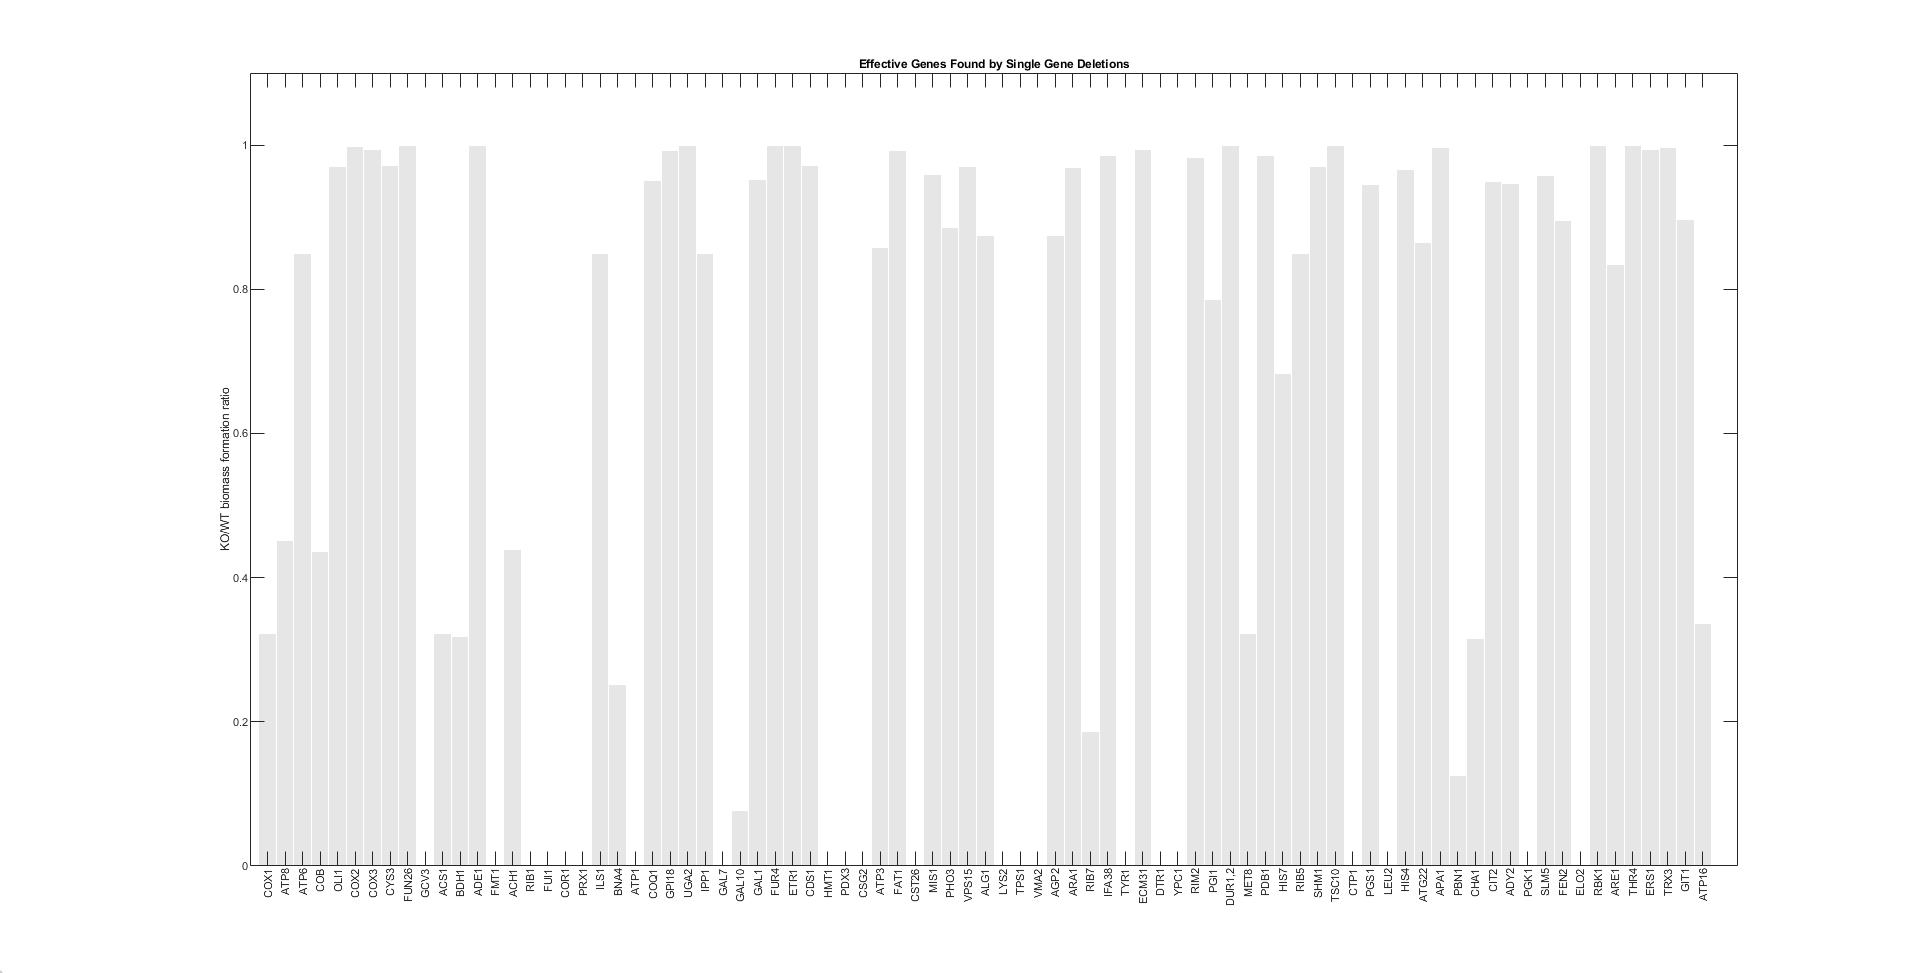
\includegraphics[width=1\columnwidth]{sgd_moma.jpg}
\end{center}
\caption[Effective genes found from the deletion analysis using MOMA]{Effective genes (not entirely essential, but their absence changes the flux distribution or value of the optimization function) obtained from single gene deletion simulations using MOMA and their effect on growth rate is plotted.}
\label{fig:sgd_moma}
\end{figure}
\hl{Explainations about knock-out strains, gene descriptions, comparison of found essential genes and their reactions corresponding to essential reactions found will be added.}

{\tiny % From here on the page will be turned sidewards.
\begin{landscape}
\begin{longtable}{p{.07\linewidth} | p{.05\linewidth} | p{.4\linewidth} | p{.4\linewidth} }
\caption[Essential genes found in Yeast8]{Total of 166 genes are found essential, meaning that their absence is crutal to model, without flux going through these genes' reactions system will not be able to grow.} \\
{Gene} & {Name} & {Name} {Description} & {Subsystem} \\
\hline
\endfirsthead
\endhead

YGL256W, YBR145W   & ADH4, ADH5  & alcohol dehydrogenase,  (acetaldehyde to ethanol), aldehyde, dehydrogenase (2-methylbutanol, 2-phenylethanol, isoamyl alcoho, isobutyl alcoho, tryptophol, 2-methylbutanol, 2-phenylethanol, isoamyl alcohol, isobutyl alcohol, tryptophol, NAD) & Gluconeogenesis, Glycolysis, Fatty acid degradation, Tyrosine metabolism,  Biosynthesis of secondary metabolites, Biosynthesis of antibiotics     \\
YER152C   & YER152C     & 2-aminoadipate transaminase   & Ubiquinone and other terpenoid-quinone biosynthesis, Cysteine and  methionine metabolism, Lysine biosynthesis, Tyrosine metabolism,  Phenylalanine metabolism, Tryptophan metabolism, Phenylalanine, tyrosine and  tryptophan biosynthesis, Biosynthesis of secondary metabolites, Biosynthesis  of antibiotics, 2-Oxocarboxylic acid metabolism, Biosynthesis of amino  acids, \\
YDR127W, YDR035W, YBR249C    & ARO1, ARO3, ARO4 & 2-deoxy-D-arabino-heptulosonate 7-phosphate synthetase, 3-deoxy-D-arabino-heptulosonate 7-phosphate synthetase & Phenylalanine, tyrosine and tryptophan biosynthesis, Biosynthesis of  secondary metabolites, Biosynthesis of antibiotics, Biosynthesis of amino  acids \\
YDR234W   & LYS4   & 2-methylcitrate dehydratase, homoacontinate hydratase  & Lysine biosynthesis, Biosynthesis of antibiotics, 2-Oxocarboxylic acid  metabolism, Biosynthesis of amino acids \\
YDR487C   & RIB3   & 3,4-dihydroxy-2-butanone-4-phosphate synthase     & Riboflavin metabolism, Biosynthesis of secondary metabolites  \\
YLR044C   & PDC1   & 3-methyl-2-oxobutanoate decarboxylase, 3-methyl-2-oxopentanoate decarboxylase, acetaldehyde condensation, indole-3-pyruvate decarboxylase,  pyruvate decarboxylase, pyruvate decarboxylase (acetoin-forming) & Gluconeogenesis, Glycolysis, Biosynthesis of secondary metabolites,  Biosynthesis of antibiotics     \\
YDL080C   & THI3   & 3-methyl-2-oxopentanoate decarboxylase, 4-methyl-2-oxopentanoate decarboxylase  & Gluconeogenesis, Glycolysis, Biosynthesis of secondary metabolites,  Biosynthesis of antibiotics     \\
YER183C   & FAU1   & 5-formethyltetrahydrofolate cyclo-ligase, 5-formyltetrahydrofolate:10-formyltetrahydrofolate isomerase   & One carbon pool by folate \\
YER037W   & PHM8   & 5'-nucleotidase (CMP), (UMP), (GMP), lysoPA phosphatase (16:0) (several lengths) & Nicotinate and nicotinamide metabolism  \\
YGR061C   & ADE6   & 5'-phosphoribosylformyl glycinamidine synthetase  & Purine metabolism, Biosynthesis of secondary metabolites, Biosynthesis of  antibiotics    \\
YIL107C   & PFK26  & 6-phosphofructo-2-kinase & Fructose and mannose metabolism    \\
YCR010C   & ADY2   & acetate transport, L-carnitine transport & Biosynthesis of amino acids     \\
YIL160C   & POT1   & acetyl-CoA C-acyltransferase (palmitoyl-CoA and other Co-As) & Fatty acid degradation, Valine, leucine and isoleucine degradation,  Biosynthesis of unsaturated fatty acids, Biosynthesis of secondary  metabolites, Biosynthesis of antibiotics, Fatty acid metabolism,  Peroxisome  \\
YAL054C   & ACS1   & acetyl-CoA synthetase    & Gluconeogenesis, Glycolysis, Pyruvate metabolism, Propanoate metabolism,  Biosynthesis of secondary metabolites, Biosynthesis of antibiotics, Carbon  metabolism \\
YAR071W   & PHO11  & acid phosphatase (secreted)   & Thiamine metabolism, Riboflavin metabolism, Cell cycle - yeast   \\
YER060W   & FCY21  & adenine transport, guanine transport, cytosine transport     &  \\
YER043C   & SAH1   & adenosylhomocysteinase   & Cysteine and methionine metabolism \\
YDR226W   & ADK1   & adenylate kinase     & Purine metabolism, Thiamine metabolism, Biosynthesis of secondary  metabolites, Biosynthesis of antibiotics     \\
YER170W   & ADK2   & adenylate kinase, adenylate kinase (GTP) & Purine metabolism, Thiamine metabolism, Biosynthesis of secondary  metabolites, Biosynthesis of antibiotics     \\
YBL030C   & PET9   & ADP/ATP transporter &  \\
YMR303C   & ADH2   & alcohol dehydrogenase (ethanol to acetaldehyde)   & Gluconeogenesis, Glycolysis, Fatty acid degradation, Tyrosine metabolism,  Biosynthesis of secondary metabolites, Biosynthesis of antibiotics     \\
YDL168W   & SFA1   & aldehyde dehydrogenase (2-methylbutanol, NAD) (2-phenylethanol, NAD)  (isoamyl alcohol, NAD) (isobutyl alcohol,  NAD) (tryptophol, NAD), formaldehyde dehydrogenase   & Gluconeogenesis, Glycolysis, Fatty acid degradation, Tyrosine metabolism,  Biosynthesis of secondary metabolites, Biosynthesis of antibiotics, Carbon  metabolism    \\
YDR481C   & PHO8   & alkaline phosphatase (dihydroneopterin)  & Thiamine metabolism, Folate biosynthesis \\
YJR152W   & DAL5   & allantoate uniport, aminoacid transport via proton symport   &  \\
YBR205W   & KTR3   & alpha 1,2-mannosyltransferase & Various types of N-glycan biosynthesis, Other types of O-glycan  biosynthesis     \\
YDR074W   & TPS2   & alpha,alpha-trehalose-phosphate synthase (UDP-forming),  trehalose-phosphatase  & Starch and sucrose metabolism  \\
YIL172C   & IMA3   & alpha-glucosidase    & Galactose metabolism, Starch and sucrose metabolism \\
YDR384C   & ATO3   & ammonia transport    &  \\
YDR354W   & TRP4   & anthranilate phosphoribosyltransferase   & Phenylalanine, tyrosine and tryptophan biosynthesis, Biosynthesis of  secondary metabolites, Biosynthesis of antibiotics, Biosynthesis of amino  acids \\
YKL211C   & TRP3   & anthranilate synthase, indole-3-glycerol-phosphate synthase  & Phenylalanine, tyrosine and tryptophan biosynthesis, Biosynthesis of  secondary metabolites, Biosynthesis of antibiotics, Biosynthesis of amino  acids \\
YDR305C   & HNT2   & Ap4A hydrolase  & Purine metabolism   \\
YDR341C   & YDR341C     & arginyl-tRNA synthetase  & Aminoacyl-tRNA biosynthesis    \\
YER052C   & HOM3   & aspartate kinase     & Glycine, serine and threonine metabolism, Monobactam biosynthesis,  Cysteine and methionine metabolism, Lysine biosynthesis, Biosynthesis of  secondary metabolites, Biosynthesis of antibiotics, 2-Oxocarboxylic acid  metabolism, Biosynthesis of amino acids  \\
YLR027C   & AAT2   & aspartate transaminase, tyrosine transaminase,  L-erythro-4-hydroxyglutamate:2-oxoglutarate aminotransferase   & Arginine biosynthesis, Alanine, aspartate and glutamate metabolism,  Cysteine and methionine metabolism, Arginine and proline metabolism, Tyrosine  metabolism, Phenylalanine metabolism, Phenylalanine, tyrosine and tryptophan  biosynthesis, Biosynthesis of secondary metabolites, Biosynthesis of  antibiotics, Carbon metabolism, 2-Oxocarboxylic acid metabolism, Biosynthesis  of amino acids   \\
YLL018C   & DPS1   & Aspartyl-tRNA synthetase & Aminoacyl-tRNA biosynthesis    \\
YJR121W   & ATP2   & ATP synthase    & Oxidative phosphorylation \\
YBR039W   & ATP3   & ATP synthase    & Oxidative phosphorylation \\
Q0085     & ATP6   & ATP synthase    & Oxidative phosphorylation \\
Q0080     & ATP8   & ATP synthase    & Oxidative phosphorylation \\
Q0130     & OLI1   & ATP synthase    & Oxidative phosphorylation \\
YEL017C-A & PMP2   & ATPase, cytosolic    & Oxidative phosphorylation, Purine metabolism, Pyrimidine metabolism   \\
YBR110W   & ALG1   & beta-1,4 mannosyltransferase  & N-Glycan biosynthesis, Various types of N-glycan biosynthesis     \\
YGL001C   & ERG26  & C-3 sterol dehydrogenase, C-3 sterol dehydrogenase (4-methylzymosterol)    & Steroid biosynthesis, Biosynthesis of antibiotics  \\
YLR056W   & ERG3   & C-5 sterol desaturase    & Steroid biosynthesis, Biosynthesis of secondary metabolites, Biosynthesis  of antibiotics \\
YJR109C   & CPA2   & carbamoyl-phosphate synthase (glutamine-hydrolysing)   & Pyrimidine metabolism, Alanine, aspartate and glutamate metabolism     \\
YER024W   & YAT2   & carnitine O-acetyltransferase & Peroxisome     \\
YBR029C   & CDS1   & CDP-diacylglycerol synthase (1-16:0, 2-16:1), ER membrane    & Glycerophospholipid metabolism, Biosynthesis of secondary metabolites,  Phosphatidylinositol signaling system \\
YDR297W   & SUR2   & ceramide-1 hydroxylase (24C), ceramide-1 hydroxylase (26C),  phytosphingosine synthesis    & Sphingolipid metabolism   \\
YKL008C   & LAC1   & ceramide-1 synthase (24C) (several lengths)   & Sphingolipid metabolism   \\
YLR133W   & CKI1   & choline kinase, ethanolamine kinase & Glycerophospholipid metabolism \\
YBR002C   & RER2   & cis-prenyltransferase step 01 to step 19 & Terpenoid backbone biosynthesis, Biosynthesis of secondary  metabolites     \\
YCR005C   & CIT2   & citrate synthase, peroxisomal & Citrate cycle (TCA cycle), Glyoxylate and dicarboxylate metabolism,  Biosynthesis of secondary metabolites, Biosynthesis of antibiotics, Carbon  metabolism, 2-Oxocarboxylic acid metabolism, Biosynthesis of amino acids   \\
YGR110W   & CLD1   & CL (1-16:0, 2-16:1, 3-16:0, 4-16:1) phospholipase (1-position),  mitochondrial membrane (Multiple reactions with varying lengths) & Glycerophospholipid metabolism \\
YHR002W   & LEU5   & coenzyme A transport, mitochondrial membrane-cytoplasm &  \\
YGL184C   & STR3   & cystathionine b-lyase    & Cysteine and methionine metabolism, Selenocompound metabolism,  Biosynthesis of secondary metabolites, Biosynthesis of amino acids  \\
YDR196C   & CAB5   & dephospho-CoA kinase     & Pantothenate and CoA biosynthesis  \\
YKL060C   & FBA1   & D-fructose 1-phosphate D-glyceraldehyde-3-phosphate-lyase,  fructose-bisphosphate aldolase, sedoheptulose 1,7-bisphosphate  D-glyceraldehyde-3-phosphate-lyase   & Gluconeogenesis, Glycolysis, Pentose phosphate pathway, Fructose and  mannose metabolism, Biosynthesis of secondary metabolites, Biosynthesis of  antibiotics, Carbon metabolism, Biosynthesis of amino acids  \\
YDL245C   & HXT15  & D-fructose transport D-mannose transport glucose transport D-sorbitol  transport L-sorbitol transport L-sorbose transport xylitol transport  D-tagatose uptake via diffusion     & Meiosis - yeast     \\
YDR345C, YHR096C, YDR343C, YDR342C & HXT3, HXT5, HXT6, HXT7 & D-fructose transport D-mannose transport glucose transport D-sorbitol  transport L-sorbitol transport L-sorbose transport xylitol transport  D-tagatose uptake via diffusion     & Meiosis - yeast     \\
YEL069C   & HXT13  & D-fructose transport, D-mannose transport, glucose transport, D-sorbitol  transport, L-sorbitol transport, L-sorbose transport, D-tagatose uptake via  diffusion & Meiosis - yeast     \\
YDL100C   & GET3   & dihydroneopterin monophosphate dephosphorylase    &  \\
YJR016C   & ILV3   & dihydroxy-acid dehydratase (2,3-dihydroxy-3-methylpentanoate)     & Valine, leucine and isoleucine biosynthesis, Pantothenate and CoA  biosynthesis, Biosynthesis of secondary metabolites, Biosynthesis of  antibiotics, 2-Oxocarboxylic acid metabolism, Biosynthesis of amino  acids \\
YJL196C   & ELO1   & elongase I (3-oxotetradecanoyl-CoA), elongase I (3-oxopalmitoyl-CoA)   & Fatty acid elongation, Biosynthesis of unsaturated fatty acids,  Biosynthesis of secondary metabolites, Fatty acid metabolism \\
YJR153W   & PGU1   & endopolygalacturonase    & Pentose and glucuronate interconversions     \\
YKR066C   & CCP1   & ferrocytochrome-c:hydrogen-peroxide oxidoreductase     & Sulfur metabolism   \\
Q0045     & COX1   & ferrocytochrome-c:oxygen oxidoreductase  & Oxidative phosphorylation, Sulfur metabolism  \\
Q0250     & COX2   & ferrocytochrome-c:oxygen oxidoreductase  & Oxidative phosphorylation, Sulfur metabolism  \\
Q0275     & COX3   & ferrocytochrome-c:oxygen oxidoreductase  & Oxidative phosphorylation, Sulfur metabolism  \\
YIL111W   & COX5B  & ferrocytochrome-c:oxygen oxidoreductase  & Oxidative phosphorylation, Sulfur metabolism  \\
YLR011W   & LOT6   & FMN reductase   &  \\
YJL155C   & FBP26  & fructose-2,6-bisphosphate 2-phosphatase  & Fructose and mannose metabolism    \\
YDR300C   & PRO1   & glutamate 5-kinase  & Arginine and proline metabolism, Carbapenem biosynthesis, Biosynthesis of  antibiotics, Biosynthesis of amino acids \\
YDL215C   & GDH2   & glutamate dehydrogenase (NAD) & Arginine biosynthesis, Alanine, aspartate and glutamate metabolism,  Taurine and hypotaurine metabolism, Nitrogen metabolism  \\
YKL104C   & GFA1   & glutamine-fructose-6-phosphate transaminase   & Alanine, aspartate and glutamate metabolism, Amino sugar and nucleotide  sugar metabolism, Biosynthesis of antibiotics  \\
YGL245W   & GUS1   & glutamyl-tRNA synthetase & Porphyrin and chlorophyll metabolism, Aminoacyl-tRNA biosynthesis,  Biosynthesis of secondary metabolites \\
YIR037W   & HYR1   & glutathione peridoxase   & Glutathione metabolism    \\
YJL212C   & OPT1   & glutathione transport, oxidized glutathione uniport    &  \\
YJR009C   & TDH2   & glyceraldehyde-3-phosphate dehydrogenase & Gluconeogenesis, Glycolysis, Biosynthesis of secondary metabolites,  Biosynthesis of antibiotics, Carbon metabolism, Biosynthesis of amino  acids \\
YHL032C   & GUT1   & glycerol kinase & Glycerolipid metabolism   \\
YGL084C   & GUP1   & glycerol transport  &  \\
YKR067W   & GPT2   & glycerol-3-phosphate acyltransferase (16:0), ER membrane,  dihydroxyacetone phosphate acyltransferase (16:0), ER membrane,  glycerol-3-phosphate acyltransferase (16:0), lipid particle, dihydroxyacetone  phosphate acyltransferase (16:0), lipid particle (all in several lengths) & Glycerolipid metabolism, Glycerophospholipid metabolism, Biosynthesis of  secondary metabolites \\
YDL022W   & GPD1   & glycerol-3-phosphate dehydrogenase (NAD) & Glycerophospholipid metabolism, Biosynthesis of secondary metabolites,  MAPK signaling pathway - yeast    \\
YDR148C   & KGD2   & glycine-cleavage complex (lipoamide), oxoglutarate dehydrogenase  (dihydrolipoamide S-succinyltransferase), oxoglutarate dehydrogenase  (lipoamide)     & Gluconeogenesis, Glycolysis, Citrate cycle (TCA cycle), Glycine, serine  and threonine metabolism, Valine, leucine and isoleucine degradation, Lysine  degradation, Tryptophan metabolism, Pyruvate metabolism, Glyoxylate and  dicarboxylate metabolism, Propanoate metabolism, One carbon pool by folate,  Biosynthesis of secondary metabolites, Biosynthesis of secondary metabolites,  Carbon metabolism \\
YJR013W   & GPI14  & GPI-anchor assembly, step 5   & Glycosylphosphatidylinositol (GPI)-anchor biosynthesis  \\
YCL052C   & PBN1   & GPI-anchor assembly, step 5   & Glycosylphosphatidylinositol (GPI)-anchor biosynthesis  \\
YDL198C   & GGC1   & GTP/GDP translocase &  \\
YDR399W   & HPT1   & guanine phosphoribosyltransferase, hypoxanthine phosphoribosyltransferase  (Hypoxanthine)  & Purine metabolism, Biosynthesis of secondary metabolites \\
YCL030C   & HIS4   & histidinol dehydrogenase, phosphoribosyl-AMP cyclohydrolase,  phosphoribosyl-ATP pyrophosphatase    & Histidine metabolism, Biosynthesis of secondary metabolites, Biosynthesis  of amino acids \\
YIL116W   & HIS5   & histidinol-phosphate transaminase   & Histidine metabolism, Tyrosine metabolism, Phenylalanine metabolism,  Phenylalanine, tyrosine and tryptophan biosynthesis, Biosynthesis of  secondary metabolites, Biosynthesis of antibiotics, Biosynthesis of amino  acids \\
YBR034C   & HMT1   & hnRNP arginine N-methyltransferase  &  \\
YDL131W   & LYS21  & homocitrate synthase     & Lysine biosynthesis, Pyruvate metabolism, Biosynthesis of antibiotics,  2-Oxocarboxylic acid metabolism, Biosynthesis of amino acids    \\
YDR453C   & TSA2   & hydrogen peroxide reductase (thioredoxin)     &  \\
YBR248C   & HIS7   & Imidazole-glycerol-3-phosphate synthase  & Histidine metabolism, Biosynthesis of secondary metabolites, Biosynthesis  of amino acids \\
YBR011C   & IPP1   & inorganic diphosphatase  & Oxidative phosphorylation \\
YDR497C   & ITR1   & inositol transport  &  \\
YDR315C   & IPK1   & inositol-1,3,4,5,6-pentakisphosphate 2-kinase     & Inositol phosphate metabolism, Phosphatidylinositol signaling system   \\
YKL004W   & AUR1   & IPC synthase (PI (1-16:0, 2-16:1) ceramide-1 (C24)) (Multiple reactions  with varying lengths)  &  \\
YER019W   & ISC1   & IPS phospholipase C & Sphingolipid metabolism   \\
YER065C   & ICL1   & isocitrate lyase     & Glyoxylate and dicarboxylate metabolism, Biosynthesis of secondary  metabolites, Carbon metabolism   \\
YBR115C   & LYS2   & L-aminoadipate-semialdehyde dehydrogenase (NADPH) & Lysine biosynthesis, Pantothenate and CoA biosynthesis, Biosynthesis of  secondary metabolites, Biosynthesis of antibiotics, Biosynthesis of amino  acids   \\
YHR072W   & ERG7   & lanosterol synthase & Steroid biosynthesis, Biosynthesis of secondary metabolites, Biosynthesis  of antibiotics \\
YEL063C   & CAN1   & L-arganine transport, orntithine transport    &  \\
    & ASP1   & L-asparaginase  & Alanine, aspartate and glutamate metabolism, Biosynthesis of secondary  metabolites    \\
YDR508C   & GNP1   & L-asparagine transport, L-cystine  transport, L-glutamine transport, L-leucine transport, L-methionine  transport, L-threonine transport, L-serine transport, asparagine transport,  methionine transport, threonine transport, serine transport &  \\
YCR075C   & ERS1   & L-cystine transport &  \\
YGR055W   & MUP1   & L-methionine transport   &  \\
YJR078W   & BNA2   & L-tryptophan:oxygen 2,3-oxidoreductase (decyclizing)   & Tryptophan metabolism     \\
YBR042C   & CST26  & lysoPI acyltransferase (1-18:0, 2-16:1), ER membrane   &  \\
YKL085W   & MDH1   & malate dehydrogenase     & Citrate cycle (TCA cycle), Cysteine and methionine metabolism, Pyruvate  metabolism, Glyoxylate and dicarboxylate metabolism, Biosynthesis of  secondary metabolites, Biosynthesis of antibiotics, Carbon metabolism     \\
YBL013W   & FMT1   & methionyl-tRNA formyltransferase    & One carbon pool by folate, Aminoacyl-tRNA biosynthesis   \\
YGR264C   & MES1   & methionyl-tRNA synthetase     & Selenocompound metabolism, Aminoacyl-tRNA biosynthesis   \\
YBR180W   & DTR1   & N,N'-diformyldityrosine transport   &  \\
YFL017C   & GNA1   & N-acetylglucosamine-6-phosphate synthase & Amino sugar and nucleotide sugar metabolism  \\
YGL067W   & NPY1   & NAD diphosphatase    & Nicotinate and nicotinamide metabolism, Peroxisome \\
YDR191W   & HST4   & NAD nucleosidase nuclear & Nicotinate and nicotinamide metabolism, Longevity regulating pathway -  multiple species   \\
YEL006W   & YEA6   & NAD transport   &  \\
YIL006W   & YIA6   & NAD transport   &  \\
YDR428C   & BNA7   & N-formyl-L-kynurenine amidohydrolase     & Tryptophan metabolism, Glyoxylate and dicarboxylate metabolism    \\
YGR010W   & NMA2   & nicotinamide-nucleotide adenylyltransferase, nicotinate-nucleotide  adenylyltransferase    & Nicotinate and nicotinamide metabolism  \\
YEL021W   & URA3   & orotidine-5'-phosphate decarboxylase     & Pyrimidine metabolism     \\
YIL145C   & PAN6   & pantothenate synthase    & beta-Alanine metabolism, Pantothenate and CoA biosynthesis, Biosynthesis  of secondary metabolites   \\
YLR060W   & FRS1   & phenylalanyl-tRNA synthetase  & Aminoacyl-tRNA biosynthesis    \\
YFL022C   & FRS2   & phenylalanyl-tRNA synthetase  & Aminoacyl-tRNA biosynthesis    \\
YGL234W   & ADE,\_7     & phopshoribosylaminoimidazole synthetase, phosphoribosylglycinamidine  synthetase & Purine metabolism, Biosynthesis of secondary metabolites, Biosynthesis of  antibiotics    \\
YCR037C   & PHO87  & phosphate transport &  \\
YJL198W   & PHO90  & phosphate transport &  \\
YGR007W   & ECT1   & phosphoethanolamine cytidyltransferase   & Phosphonate and phosphinate metabolism, Glycerophospholipid  metabolism     \\
YKL127W   & PGM1   & phosphoglucomutase, phosphopentomutase   & Gluconeogenesis, Glycolysis, Pentose phosphate pathway, Galactose  metabolism, Purine metabolism, Starch and sucrose metabolism, Amino sugar and  nucleotide sugar metabolism, Biosynthesis of secondary metabolites,  Biosynthesis of antibiotics   \\
YCR012W   & PGK1   & phosphoglycerate kinase  & Gluconeogenesis, Glycolysis, Biosynthesis of secondary metabolites,  Biosynthesis of antibiotics, Carbon metabolism, Biosynthesis of amino  acids \\
YKR072C   & SIS2   & phosphopantothenoylcysteine decarboxylase     & Pantothenate and CoA biosynthesis  \\
YAR015W   & ADE1   & phosphoribosyl amino imidazolesuccinocarbozamide synthetase  & Purine metabolism, Biosynthesis of secondary metabolites, Biosynthesis of  antibiotics    \\
YDR007W   & TRP1   & phosphoribosylanthranilate isomerase     & Phenylalanine, tyrosine and tryptophan biosynthesis, Biosynthesis of  secondary metabolites, Biosynthesis of antibiotics, Biosynthesis of amino  acids \\
YER026C   & CHO1   & PS synthase (1-16:0, 2-16:1), ER membrane (several lengths)  & Glycine, serine and threonine metabolism, Glycerophospholipid metabolism,  Biosynthesis of secondary metabolites   \\
YBR221C   & PDB1   & pyruvate dehydrogenase   & Gluconeogenesis, Glycolysis, Citrate cycle (TCA cycle), Glycine, serine  and threonine metabolism, Valine, leucine and isoleucine degradation,  Pyruvate metabolism, Glyoxylate and dicarboxylate metabolism, Propanoate  metabolism, Biosynthesis of secondary metabolites, Biosynthesis of  antibiotics, Carbon metabolism \\
YGR193C   & PDX1   & pyruvate dehydrogenase   & Gluconeogenesis, Glycolysis, Citrate cycle (TCA cycle), Glycine, serine  and threonine metabolism, Valine, leucine and isoleucine degradation,  Pyruvate metabolism, Glyoxylate and dicarboxylate metabolism, Propanoate  metabolism, Biosynthesis of secondary metabolites, Biosynthesis of  antibiotics, Carbon metabolism \\
YGL080W   & MPC1   & pyruvate transport  &  \\
YIL020C   & HIS6   & raffinose invertase,  1-(5-phosphoribosyl)-5-{[}(5-phosphoribosylamino)methylideneamino)imidazole-4-carboxamide  isomerase   & Histidine metabolism, Biosynthesis of secondary metabolites, Biosynthesis  of amino acids \\
YBR256C   & RIB5   & riboflavin synthase & Riboflavin metabolism, Biosynthesis of secondary metabolites  \\
YBR132C   & AGP2   & spermidine transport     &  \\
YKR053C   & YSR3   & sphingoid base-phosphate phosphatase (phytosphingosine 1-phosphate),  sphingoid base-phosphate phosphatase (sphinganine 1-phosphatase)  & Sphingolipid metabolism   \\
YJL045W   & YJL045W     & succinate dehydrogenase (ubiquinone-6)   & Citrate cycle (TCA cycle), Oxidative phosphorylation, Biosynthesis of  secondary metabolites, Biosynthesis of antibiotics, Carbon metabolism     \\
YIL162W   & SUC2   & sucrose hydrolyzing enxyme    & Galactose metabolism, Starch and sucrose metabolism \\
YJR137C   & MET5   & sulfite reductase (NADPH2)    & Sulfur metabolism   \\
YMR313C   & TGL3   & TAG lipase (1-16:0, 2-16:1, 3-16:0), lipid particle, DAG lipase (1-16:0,  2-16:1), lipid particle, lysoPE (1-16:0) oleoyl-CoA acyltransferase, lipid  particle (all in several lengths)   & Steroid biosynthesis, Glycerolipid metabolism, Glycerophospholipid  metabolism, Biosynthesis of secondary metabolites    \\
YKL132C   & RMA1   & tetrahydrofolate:L-glutamate gamma-ligase (ADP-forming) & Folate biosynthesis \\
YGR096W   & TPC1   & thiamine diphosphate transport &  \\
YDL015C   & TSC13  & trans-2-enoyl-CoA reductase (n-C14:0CoA) (several lengths)   & Fatty acid elongation, Biosynthesis of unsaturated fatty acids,  Biosynthesis of secondary metabolites, Fatty acid metabolism \\
YGL026C   & TRP5   & tryptophan synthase (indoleglycerol phosphate)    & Glycine, serine and threonine metabolism, Phenylalanine, tyrosine and  tryptophan biosynthesis, Biosynthesis of secondary metabolites, Biosynthesis  of antibiotics, Biosynthesis of amino acids   \\
Q0105     & COB    & ubiquinol:ferricytochrome c reductase    & Oxidative phosphorylation, Sulfur metabolism  \\
YJL166W   & QCR8   & ubiquinol:ferricytochrome c reductase    & Oxidative phosphorylation, Sulfur metabolism  \\
YEL024W   & RIP1   & ubiquinol:ferricytochrome c reductase    & Oxidative phosphorylation, Sulfur metabolism  \\
YDL103C   & QRI1   & UDP-N-acetylglucosamine diphosphorylase  & Amino sugar and nucleotide sugar metabolism, Biosynthesis of  antibiotics   \\
YBL042C   & FUI1   & uridine transport, deoxyuridine transport     &  \\
YKL035W   & UGP1   & UTP-glucose-1-phosphate uridylyltransferase   & Pentose and glucuronate interconversions, Galactose metabolism, Starch  and sucrose metabolism, Amino sugar and nucleotide sugar metabolism,  Biosynthesis of antibiotics \\
YJR148W   & BAT2   & valine transaminase, leucine transaminase, isoleucine transaminase,  2-oxo-4-methyl-3-carboxypentanoate decarboxylation,  2-keto-4-methylthiobutyrate transamination  & Cysteine and methionine metabolism, Valine, leucine and isoleucine  degradation, Valine, leucine and isoleucine biosynthesis, Pantothenate and  CoA biosynthesis, Biosynthesis of secondary metabolites, Biosynthesis of  antibiotics, 2-Oxocarboxylic acid metabolism, Biosynthesis of amino  acids \\
YLL052C   & AQY2   & water diffusion, H2O transport,  3-dehydroquinate dehydratase, 3-dehydroquinate synthase, 3-phosphoshikimate  1-carboxyvinyltransferase, shikimate dehydrogenase, shikimate kinase  &  \\
YJR133W   & XPT1   & xanthine phosphoribosyltransferase  &  \\
YFL001W   & DEG1   & yUMP synthetase &  \\
YKL152C   & GPM1   & & Gluconeogenesis, Glycolysis, Glycine, serine and threonine metabolism,  Biosynthesis of secondary metabolites, Biosynthesis of antibiotics, Carbon  metabolism, Biosynthesis of amino acids   \\
YCR036W   & RBK1   & & Pentose phosphate pathway
\label{table:essential_genes}
\end{longtable}
\end{landscape} }


\section{Expression Data Analysis}
\hl{GSE numbers, experimental conditions, data normalization, gene enrichment analysis, comparison with essential genes in the model...}
\section{Integration of Expression Data Into Model}
\hl{Used method and its mathematical explaination on flux bounds...}
